%  LaTeX support: latex@mdpi.com 
%  In case you need support, please attach all files that are necessary for compiling as well as the log file, and specify the details of your LaTeX setup (which operating system and LaTeX version / tools you are using).

% You need to save the "mdpi.cls" and "mdpi.bst" files into the same folder as this template file.

%=================================================================
\documentclass[remotesensing,article,submit,moreauthors,pdftex,10pt,a4paper]{mdpi} 
%
%--------------------
% Class Options:
%--------------------
% journal
%----------
% Choose between the following MDPI journals:
% actuators, addictions, admsci, aerospace, agriculture, agronomy, algorithms, animals, antibiotics, antibodies, antioxidants, applsci, arts, asi, atmosphere, atoms, axioms, batteries, bdcc, behavsci, beverages, bioengineering, biology, biomedicines, biomimetics, biomolecules, biosensors, brainsci, buildings, carbon, cancers, catalysts, cells, ceramics, challenges, chemengineering, chemosensors, children, chromatography, climate, coatings, colloids, computation, computers, condensedmatter, cosmetics, cryptography, crystals, cybersecurity, data, dentistry, designs, diagnostics, diseases, diversity, econometrics, economies, education, electrochemistry, electronics, energies, entropy, environments, epigenomes, est, fermentation, fibers, fire, fishes, fluids, foods, forests, fractalfract, futureinternet, galaxies, games, gastrointestdisord, gels, genealogy, genes, geosciences, geriatrics, hazardousmatters, healthcare, heritage, highthroughput, horticulturae, humanities, hydrology, informatics, information, infrastructures, inorganics, insects, instruments, ijerph, ijfs, ijms, ijgi, ijtpp, inventions, j, jcdd, jcm, jcs, jdb, jfb, jfmk, jimaging, jof, jintelligence, jlpea, jmmp, jmse, jpm, jrfm, jsan, land, languages, laws, life, literature, logistics, lubricants, machines, magnetochemistry, make, marinedrugs, materials, mathematics, mca, mti, medsci, medicines, membranes, metabolites, metals, microarrays, micromachines, microorganisms, minerals, modelling, molbank, molecules, mps, nanomaterials, ncrna, neonatalscreening, nitrogen, nutrients, ohbm, particles, pathogens, pharmaceuticals, pharmaceutics, pharmacy, philosophies, photonics, plants, plasma, polymers, preprints, proceedings, processes, proteomes, publications, quaternary, qubs, recycling, religions, remotesensing, resources, risks, robotics, safety, scipharm, sensors, separations, sexes, sinusitis, socsci, societies, soils, sports, standards, surgeries, sustainability, symmetry, systems, technologies, toxics, toxins, tropicalmed, universe, urbansci, vaccines, vetsci, vibration, viruses, vision, water, wem
%---------
% article
%---------
% The default type of manuscript is article, but can be replaced by: 
% abstract, addendum, article, benchmark, book, bookreview, briefreport, casereport, changes, comment, commentary, communication, conceptpaper, correction, conferenceproceedings, conferencereport, expressionofconcern, meetingreport, creative, datadescriptor, discussion, editorial, essay, erratum, hypothesis, interestingimages, letter, meetingreport, newbookreceived, opinion, obituary, projectreport, reply, reprint, retraction, review, perspective, protocol, shortnote, supfile, technicalnote, viewpoint
% supfile = supplementary materials
% protocol: If you are preparing a "Protocol" paper, please refer to http://www.mdpi.com/journal/mps/instructions for details on its expected structure and content.
%----------
% submit
%----------
% The class option "submit" will be changed to "accept" by the Editorial Office when the paper is accepted. This will only make changes to the frontpage (e.g. the logo of the journal will get visible), the headings, and the copyright information. Also, line numbering will be removed. Journal info and pagination for accepted papers will also be assigned by the Editorial Office.
%------------------
% moreauthors
%------------------
% If there is only one author the class option oneauthor should be used. Otherwise use the class option moreauthors.
%---------
% pdftex
%---------
% The option pdftex is for use with pdfLaTeX. If eps figures are used, remove the option pdftex and use LaTeX and dvi2pdf.

%=================================================================
\firstpage{1} 
\makeatletter 
\setcounter{page}{\@firstpage} 
\makeatother 
\articlenumber{x}
\doinum{10.3390/------}
\pubvolume{xx}
\pubyear{2017}
\copyrightyear{2017}
\externaleditor{Academic Editor: name}
\history{Received: date; Accepted: date; Published: date}

\usepackage{gensymb}
\usepackage{natbib}
\usepackage{tabulary}
\usepackage{multirow}
\usepackage{boldline}

\usepackage[british]{babel}

\usepackage{amsmath}
\usepackage{amsthm}
\usepackage{amsfonts}
\usepackage{amssymb}

\usepackage{booktabs}
\usepackage{tabularx}
\usepackage{multirow}
\usepackage{graphicx}

\usepackage[font=footnotesize]{caption}
\usepackage[font=footnotesize]{subcaption}

\definecolor{mygreen}{rgb}{0.1, 0.6, 0.4}
\newcommand{\added}[1]{\color{mygreen}{#1} \color{black}}
\newcommand{\changed}[1]{\color{red}{#1} \color{black}}

\newcommand{\adjrsq}{adjusted $R^2$}
\newcommand{\rmsecv}{RMSE$_{cv}$}
\newcommand{\mha}{m$^3$/ha}
\newcommand{\bwi}{BWI3}
\newcommand{\psynth}{PSYNTH}
\newcommand{\psmall}{PSMALL}
\newcommand{\extpsynth}{EXTPSYNTH}
\newcommand{\meanheight}{\textit{meanheight}}
\newcommand{\stddev}{\textit{stddev}}
\newcommand{\treespecies}{\textit{treespecies}}
\newcommand{\alsyear}{\textit{ALSyear}}
\newcommand{\var}{\mathbb{V}}
\newcommand{\EX}{\mathbb{E}}

%------------------------------------------------------------------
% The following line should be uncommented if the LaTeX file is uploaded to arXiv.org
%\pdfoutput=1

%=================================================================
% Add packages and commands here. The following packages are loaded in our class file: fontenc, calc, indentfirst, fancyhdr, graphicx, lastpage, ifthen, lineno, float, amsmath, setspace, enumitem, mathpazo, booktabs, titlesec, etoolbox, amsthm, hyphenat, natbib, hyperref, footmisc, geometry, caption, url, mdframed, tabto, soul, multirow, microtype, tikz

%=================================================================
%% Please use the following mathematics environments: Theorem, Lemma, Corollary, Proposition, Characterization, Property, Problem, Example, ExamplesandDefinitions, Hypothesis, Remark, Definition
%% For proofs, please use the proof environment (the amsthm package is loaded by the MDPI class).

%=================================================================
% Full title of the paper (Capitalized)
\Title{A double-sampling extension of the German National Forest Inventory for design-based small area estimation on forest district levels}

% Author Orchid ID: enter ID or remove command
\newcommand{\orcidauthorA}{0000-0002-6367-2256} % Add \orcidA{} behind the author's name
%\newcommand{\orcidauthorB}{0000-0000-000-000X} % Add \orcidB{} behind the author's name

% Authors, for the paper (add full first names)
\Author{Andreas Hill $^{1,}$*\orcidA{}, Daniel Mandallaz $^{1}$ and Joachim Langshausen $^{2}$}

% Authors, for metadata in PDF
\AuthorNames{Andreas Hill, Daniel Mandallaz and Joachim Langshausen}

% Affiliations / Addresses (Add [1] after \address if there is only one affiliation.)
\address{%
	$^{1}$ \quad Department of Environmental Systems Science, ETH Zurich, 8092 Zurich, Switzerland; mdaniel@retired.ethz.ch (D.M.)\\
	$^{2}$ \quad State Forest Service Rhineland-Palatinate, 56281 Emmelshausen, Germany; Joachim.Langshausen@wald-rlp.de}

% Contact information of the corresponding author
\corres{Correspondence: andreas.hill@usys.ethz.ch; Tel.: +x-xxx-xxx-xxxx}



% Abstract (Do not insert blank lines, i.e. \\) 
\abstract{The German National Forest Inventory consists of a systematic grid of permanent sample plots and provides a reliable evidence-based assessment of the state and the development of Germany's forests on national and federal state level in a 10 year interval. However, the data have yet been scarcely used for estimation on smaller management levels such as forest districts due to insufficient sample sizes within the area of interests and the implied large estimation errors. In this study, we present a double-sampling extension to the existing German National Forest Inventory (NFI) that allows for the application of recently developed design-based small area regression estimators. We illustrate the implementation of the estimation procedure and evaluate its potential for future large-scale operational application by the example of timber volume estimation on two small-scale management levels (45 and 405 forest district units respectively) over the entire area of the federal German state of Rhineland-Palatinate. An airborne laserscanning (ALS) derived canopy height model and a tree species classification map based on satellite data were used as auxiliary data in an ordinary least square regression model to produce the timber volume predictions. The results support that the suggested double-sampling procedure can substantially increase estimation precision on both management levels: the two-phase estimators were able to reduce the variance of the one-phase simple random sampling estimator by 43\% and 25\% on average for the two management levels respectively.}

% Keywords
\keyword{National forest inventory, small area estimation, forest districts, double sampling for regression within strata, cluster sampling, canopy height model, tree species classification}

% The fields PACS, MSC, and JEL may be left empty or commented out if not applicable
%\PACS{J0101}
%\MSC{}
%\JEL{}

%%%%%%%%%%%%%%%%%%%%%%%%%%%%%%%%%%%%%%%%%%
% Only for the journal Applied Sciences:
%\featuredapplication{Authors are encouraged to provide a concise description of the specific application or a potential application of the work. This section is not mandatory.}
%%%%%%%%%%%%%%%%%%%%%%%%%%%%%%%%%%%%%%%%%%

%%%%%%%%%%%%%%%%%%%%%%%%%%%%%%%%%%%%%%%%%%
% Only for the journal Data:
%\dataset{DOI number or link to the deposited data set in cases where the data set is published or set to be published separately. If the data set is submitted and will be published as a supplement to this paper in the journal Data, this field will be filled by the editors of the journal. In this case, please make sure to submit the data set as a supplement when entering your manuscript into our manuscript editorial system.}

%\datasetlicense{license under which the data set is made available (CC0, CC-BY, CC-BY-SA, CC-BY-NC, etc.)}

%\setcounter{secnumdepth}{4}
%%%%%%%%%%%%%%%%%%%%%%%%%%%%%%%%%%%%%%%%%%

\begin{document}
%%%%%%%%%%%%%%%%%%%%%%%%%%%%%%%%%%%%%%%%%%
%% Only for the journal Gels: Please place the Experimental Section after the Conclusions

%%%%%%%%%%%%%%%%%%%%%%%%%%%%%%%%%%%%%%%%%%
%\setcounter{section}{-1} %% Remove this when starting to work on the template.
%\section{How to Use this Template}
%The template details the sections that can be used in a manuscript. Note that the order and names of article sections may differ from the requirements of the journal (e.g. the positioning of the Materials and Methods section). Please check the instructions for authors page of the journal to verify the correct order and names. For any questions, please contact the editorial office of the journal or support@mdpi.com. For LaTeX related questions please contact Janine Daum at latex-support@mdpi.com.


\section{Introduction}
\label{sec:intro}

The German National Forest Inventory (NFI) provides reliable evidence-based and accurate information of the current state and the development of Germany's forest over time. The NFI thereby has the responsibility to satisfy various information needs including reporting to public and state forestry administrations, wood-based industries and the public on the national level, as well as to the Food and Agriculture Organization of the United Nations (FAO) and to the United Nations Framework Convention on Climate Change (UNFCC) on the international level \citep{polley2010intomppo}. The current design of the German NFI rests solely upon a terrestrial cluster inventory that is carried out at sample locations systematically distributed over the entire forested area of Germany. In order to cover a large area of 114'191 km$^2$ \citep{bwi3}, the sample size has been specifically chosen to satisfy high estimation accuracies for forest attributes on the national and federal state levels. However, sample sizes often drop dramatically when entering spatial units below the federal state level. This is particularly true for forest management levels such as forest districts for which the estimation uncertainties turn out to be unacceptably large due to the very limited number of sample plots within these units. For this reason, the German NFI data have not yet been extensively incorporated into operational planning on forest district management levels. In most German federal states, management strategies are thus still based on expert judgements from time-consuming standwise forest inventories (SFI), which are prone to systematic deviations \cite{kulievsis2016} and do not provide any measure of uncertainty.\par

Some German federal states, such as Lower Saxony, have approached this problem by establishing a regional Forest District Inventory (FDI) carried out for forests owned by the state forest enterprise with a much higher sampling density than used by the NFI in order to scientifically base their regional management strategies on quantitative and accurate information \citep{bockmann1998}. However, such FDIs are cost-intensive and, facing increasing restrictions in budget and staff resources, there has been a need for more cost-efficient inventory methods \citep{vonluepke2013}. One method which has proven to be efficient is double- or two-phase sampling \citep{sarndal2003, gregoire2007, kohl2006, mandallaz2008}. Double-sampling incorporates less expensive auxiliary information and can be used to either increase estimation precision under a fixed terrestrial sample size, or maintain estimation precision under reduced terrestrial sample size. Double-sampling procedures have already been used for stratification in the FDI of Lower Saxony \citep{saborowski2010}, and \citet{grafstrom2017a} illustrated how to use the auxiliary information to determine optimised balanced terrestrial sample designs. Recent studies have extended double-sampling to triple-sampling estimation methods using auxiliary information derived at two different sampling intensities. An example can be found in \citet{vonLuepke2012} who illustrated an extension of the existing two-phase FDI of Lower Saxony to a three-phase design that uses updates of past inventory data as additional auxiliary information and allows for a significant reduction of the terrestrial sample size in intermediate inventories. Another example is \citet{massey2014a} who developed a triple-sampling extension based on the ideas of \citet{mandallaz2013c} for the Swiss NFI that can significantly reduce the increase in estimation uncertainty caused by the new annual inventory design.\par

Two-phase and three-phase samplings techniques have also been applied to small area estimation (SAE). SAE techniques address the situation where the number of samples within a subunit, or small area (SA), of the entire sampling frame is too small to provide reliable estimates for that unit. A broad range of SA estimators used in forest inventories \citep{kohl2006} originally comes from official statistics. One such method that is commonly applied is known as indirect estimation \citep{rao2015}, where statistical models are used to convert auxiliary information into predictions of the target variable that is rarely or not observed in the small area. These models are trained using data from outside the small area in order to "borrow strength" from areas where information is available. Of numerous applications of SAE in forestry \citep{breidenbach2012, goerndt2011, steinmann2013, mandallaz2013b}, most use unit-level models, i.e. the inventory plot is the unit of the response variable in the training data used for the model fit. Such unit-level models have been intensively investigated for timber volume estimation using various remote sensing auxiliary data \citep{koch2010, naesset2014inmaltamo}. Other studies have investigated area-level models, where the auxiliary information is only provided on the SA level \citep{magnussen2017}. Some studies have illustrated that even NFI data derived under low sampling densities can still be used to provide acceptable precision of small area estimates on much smaller management levels. One example is \citet{breidenbach2012} who used data from the Norwegian NFI to make small area estimation for standing timber volume for 14 municipalities where the number of NFI samples within these areas were between 1 and 35. The estimation errors under the applied model-dependent and design-based small area estimators turned to be markedly smaller than under the standard one-phase estimator. Another example is \citet{magnussen2014} who recently used the Swiss NFI data to estimate timber volume within 108 Swiss forest districts with sample sizes between 9 and 206. Similar studies using German NFI data for small area estimation have been lacking.\par

The objective of this study was to investigate whether the application of latest design-based small area estimation methods allow to use the German NFI data to produce estimates of acceptable precision on two forest district levels. The methods were tested in the German federal state Rhineland-Palatinate. Three types of model-assisted design-based small area regression estimators were used to derive point and variance estimates of mean standing timber volume for 45 and 405 forest management units on the two respective district levels. The SA-estimators we considered were the \textit{pseudo-small}, \textit{extended pseudo-synthetic} and the \textit{pseudo-synthetic} design-based small area estimator suggested by \citet{mandallaz2013a} and \citet{ mandallaz2013b}. Auxiliary data consisted of a canopy height model (CHM) obtained from a countrywide airborne laser scanning (ALS) and a tree species classification map to be used for regression within tree species strata. The estimation precisions were compared to those obtained by the standard one-phase estimator for cluster sampling under simple random sampling. The chosen double-sampling estimators were selected for several reasons: \textbf{(i)} the design-based framework relaxes dependencies on the regression model assumptions which seemed appropriate facing severe quality restrictions in the ALS data; \textbf{(ii)} the estimators can be used with \textit{non-exhaustive}, i.e. non wall-to-wall, auxiliary information; \textbf{(iii)} all estimators are explicitly formulated for cluster sampling which has not yet been the case for frequently used model-dependent estimators; and \textbf{(iv)} the asymptotically unbiased g-weight variance partially accounts for estimating the regression coefficients on the same sample used for estimation (\textit{internal model approach}) and is also robust under heteroscedasticity of the model residuals. The results from this study were considered to provide valuable information about the potential of the suggested small area estimation procedure and the incorporated auxiliary information for future operational large scale application.\par

%---------------------------------------------------------------------------------------------------------%
% ---------------------------------- Materials and Methods ---------------------------------------------- %

\section{Terrestrial sampling design of the German NFI}
\label{sec:germanNFI}

The German NFI is a periodic inventory that is carried out every 10 years over the entire forest area of Germany. The most recent inventory (BWI3) was conducted in 2011 and 2012. While information was originally gathered on a systematic 4x4 km grid, some federal states such as Rhineland-Palatinate have switched to a densified 2x2 km grid. The German NFI uses a cluster sampling design, which means that a sample unit consists of at most four sample locations (also referred to as \textit{sample plots}) that are arranged in a square, called \textit{cluster}, with a side length of 150 metres. The number of plots per cluster can vary between 1 and 4 depending on forest/non-forest decisions by the field crews on the individual plot level \citep{bwi3_aufn}. In the field survey of the BWI3, sample trees for timber volume estimation are selected according to the angle count sampling technique \citep{bitterlich1984}, using a basal area factor ($BAF$) of 4 that is respectively adjusted for sample trees at the forest boundary by a geometric intersection of the boundary transect with the individual tree's inclusion circle \citep{bwi3_aufn}. A further inventory threshold for a tree to be recorded is a diameter at breast height ($DBH$) of at least 7 cm. For each sample tree that is selected by this procedure, the DBH, the absolute tree height, the tree diameter at 7 m ($D7$) and the tree species is measured and used to estimate the volume at the tree level. These volume estimates are based on the application of tree species specific taper curves that are adjusted to the set of diameters and corresponding height measurements taken from the respective sample tree \citep{kublin2013}.


% ++++++++++++ %
\section{Double sampling in the infinite population approach}
\label{sec:inf_pop}

 \subsubsection{One- and Two-Phase Sampling in the Infinite Population Approach}

The estimators used in this study have been proposed by \citep{mandallaz2013a,mandallaz2013b} and derive their mathematical properties under the so-called infinite population approach. Therefore, we shall first provide a short introduction into this general estimation framework. We start by assuming that the population $P$ of trees $i \in 1,2, ..., N$ within a forest of interest $F$ is exactly defined, and each tree $i$ has a response variable $Y_i$ (e.g. its timber volume) that can be used to define the population mean $Y$ (e.g., the average timber volume per unit area) over $F$. Since a full census of all tree population individuals is almost never feasible, $Y$ has to be estimated based on a sample. In the infinite population approach this sample is a set of points or locations $x$ distributed independently and uniformly over the set of all possible points in $F$. Each point $x$ has an associated local density $Y(x)$ (e.g., the timber volume per unit area) whose spatial distribution is given by a fixed (i.e. non stochastic) piecewise constant function. The population mean $Y$ is mathematically equivalent to the integral of the local density function surface divided by the surface area of $F$, $\lambda(F)$, i.e. $Y=\frac{1}{N} \sum_{i=1}^{N}Y_i=\frac{1}{\lambda(F)}\int_{F}Y(x)dx$, and thus the population mean $Y$ corresponds to a spatial mean. Since the actual local density function is unobserved in its entirety, one estimates $Y$ by taking a sample $s_2$ consisting of $n_2$ points and measuring each of their respective local densities. This sampling procedure is often referred to as \textit{one-phase sampling} (OPS) and $s_2$ is referred to as the terrestrial inventory. In contrast to the one-phase approach, \textit{two-phase} or \textit{double-sampling} procedures use information from two nested samples (phases). Practically speaking, the terrestrial inventory $s_2$ is embedded in a large phase $s_1$ comprising $n_1$ sample locations that each provide a set of explanatory variables described by the column vector $\pmb{Z}(x)=(z(x)_1, z(x)_2,...,z(x)_p)^{\top}$ at each point $x \in s_1$. These explanatory variables are derived from auxiliary information that is available in high quantity within the forest $F$. For every $x \in s_1$, $\pmb{Z}(x)$ is transformed into a prediction $\hat{Y}(x)$ of $Y(x)$ using the choice of some prediction model. The basic idea of this method is to boost the sample size by providing a large sample of less precise but cheaper predictions of $Y(x)$ in $s_1$ and to correct any possible model bias, i.e., $\EX{(Y(x)-\hat{Y}(x))}$, using the subsample of terrestrial inventory units where the value of $Y(x)$ is observed. In this context, it is also important to note that the response and auxiliary variables are assumed to be error-free and the resulting errors for the point estimates reflect only the uncertainty due to sampling.


% ----------------------------------------------------------------------- %
% ----------------------------------------------------------------------- %
\section{Estimators}
\label{sec:estimators}


% ++++++++++++ %
\subsection{Design-based one-phase estimator for cluster sampling (SRS)}
\label{sec:srs_estimator}

The one-phase estimator for cluster sampling (SRS) constitutes the \textit{status quo} that is currently applied under the existing one-phase sampling design of the German NFI in order to obtain point and variance estimates for the mean timber volume of a given estimation unit. In order to provide all estimators in the infinite population framework and ensure a consistent terminology with the two-phase estimators in Section \ref{sec:SAestimators}, we will introduce the SRS estimator that is applied in the BWI3 algorithms \citep{bwi3_ausw} in the form given in \citet{mandallaz2008} and \citet{mandallaz2016}.\par 
In order to calculate the local density $Y_{c}(x)$ at the cluster level, a cluster is defined as consisting of $M$ sample locations (in the BWI3, we have $M=4$ ) where $M-1$ sample locations $x_2, ..., x_M$ are created close to the cluster origin $x_1$ by adding a fixed set of spatial vectors $e_2, ..., e_M$ to $x_1$. The actual number of plots per cluster, $M(x)$, is a random variable due to the uniform distribution of $x_l$ ($l=1, ..., M$) in the forest $F$ and to the forest/non-forest decision for each sample location $x_l$:

\begin{equation}\label{eq:Mx}
M(x)=\sum_{l=1}^{M}I_{F}(x_l) \hspace{3ex} \text{where} \hspace{3ex} I_F(x_l)=\begin{cases}&1 \text{ if $x_l \in F$}\\
&0 \text{ if $x_l\not\in F$}
\end{cases}
\end{equation}

The local density on cluster level $Y_{c}(x)$, which is in our case the timber volume per hectare, is then defined as the average of the individual sample plot densities $Y(x_l)$:

\begin{equation}\label{eq:locdens_clust}
Y_{c}(x) = \frac{\sum_{l=1}^{M} I_{F}(x_{l}) Y(x_l)}{M(x)}
\end{equation}

The local density $Y(x_l)$ on individual sample plot level was calculated according to the description in \citet{mandallaz2008}, which can be rewritten for angle-count sampling technique applied in the BWI3. The general form of $Y(x)$ in \citet{mandallaz2008} is given as the Horwitz-Thompson estimator 

%\begin{equation}\label{locdens_plot}
%Y(x)= \sum_{i=1}^{F}\frac{I_{i}(x)Y_i}{\varPi_{i}\lambda(F)} = \sum_{i \in s_{2}(x)}\frac{Y_i}{\varPi_{i}\lambda(F)}
%\end{equation}

\begin{equation}\label{eq:locdens_plot}
Y(x_l)=\sum_{i \in s_{2}(x_l)}\frac{Y_i}{\pi_{i}\lambda(F)}
\end{equation}

\noindent where $Y_i$ is in our case the timber volume of the tree $i$ recorded at sample location $x$ in m$^3$. Each tree has an inclusion probability $\pi_{i}$ that is well defined as the proportion of its inclusion circle area $\lambda(K_i)$ within the forest area $\lambda(F)$, i.e. via their geometric intersection:

%with the binary indicator variable $Ii$ for the $i$th tree defined as
%
%\begin{equation}\label{1stage}
%I_i(x)=\begin{cases}&1 \text{ if $x \in K_i$}\\
%&0 \text{ if $x\not\in K_i$}
%\end{cases}
%\end{equation}

\begin{equation}\label{locdens_plot_1}
\pi_{i} = \frac{\lambda(K_i \cap F)}{\lambda(F)}
\end{equation}

The radius $R_i$ of the tree's inclusion circle $K_i$ is given by $R_i = DBH_{i}/cf_{i,corr}$ (also referred to as \textit{limiting distance}), where $cf_{i,corr}$ is the original counting factor $cf$ corrected for potential boundary effects at the forest border. In case of angle-count sampling, we can rewrite $\pi_{i}$ as

\begin{equation}\label{eq:locdens_plot_2}
\pi_{i} = \frac{G_i}{cf_{i,corr}\lambda(F)}
\end{equation}

\noindent since the intersection area $\lambda(K_i \cap F)/\lambda(F)$ can be expressed using the trees basal area $G_i$ (in m$^2$) and the corrected counting factor:

\begin{equation}\label{eq:locdens_plot_3}
\lambda(K_i \cap F) = \frac{G_i}{cf_{i, corr}} \hspace{3ex} \text{where} \hspace{3ex} cf_{i,corr} = cf\frac{\lambda(K_i)}{\lambda(K_i \cap F)}
\end{equation}

Eq. \ref{eq:locdens_plot_2} in Eq. \ref{eq:locdens_plot} yields the rewritten form of $Y(x_l)$ for angle count sampling that conforms to the definition used in the BWI3 algorithms \citep{bwi3_ausw}:

\begin{equation}\label{eq:locdens_plot_4}
Y(x_l)= \sum_{i \in s_{2}(x_l)} \frac{cf_{i, corr}Y_i}{G_i} = \sum_{i \in s_{2}(x_l)} nha_{i}{Y_i}
\end{equation}

\noindent where $nha_i$ is the number of trees per hectare represented by tree $i$. The local densities on cluster level can then be used to derive the estimated spatial mean $\hat{\bar{Y}}_c$ and its estimated variance $\hat{\var}(\hat{\bar{Y}}_c)$ for any given spatial unit for which $n_2 \geq 2$ ($n_2$ denoting the number of clusters):

\begin{subequations}\label{eq:srs_est_clusters}
	\begin{align}
	\hat{\bar{Y}}_c &= \frac{\sum_{x \in s_2} M(x) Y_{c}(x)}{\sum_{x \in s_2} M(x)} \\
	\hat{\var}(\hat{\bar{Y}}_c) &= \frac{1}{n_2(n_2 - 1)}\sum_{x \in s_2}\Big(\frac{M(x)}{\bar{M_2}}\Big)^2(Y_{c}(x) - \hat{\bar{Y}}_c)^2
	\end{align}
\end{subequations}

with $\bar{M_2}=\frac{\sum_{x \in s_{2}}M(x)}{n_{2}}$.

% \newpage

% +++++++++++++++++++++++++++++ %
\subsection{Design-based small area regression estimators for cluster sampling}
\label{sec:SAestimators}

All three considered small area estimators use ordinary least square (OLS) regression models to produce predictions of the local density $Y_{c}(x)$ directly on the cluster level $c$. We consider the internal model approach, where the estimators take into account that the regression coefficients on the cluster level were fitted using the same sample used for estimation. To apply this to small area estimation, the vector of estimated regression coefficients on the cluster level is found by "borrowing strength" from the entire terrestrial sample $s_2$ of the current inventory:

\begin{subequations}\label{normequ_simple_cluster}
	\begin{align}
	\hat{\pmb{\beta}}_{c,s_2} &= \pmb{A}_{c,s_2}^{-1} \Big(\frac{1}{n_2}\sum_{x\in{s_2}}M(x)Y_{c}(x)\pmb{Z}_{c}(x)\Big) \\
	\pmb{A}_{c,s_2} &=\frac{1}{n_2}\sum_{x\in{s_2}}M(x)\pmb{Z}_{c}(x)\pmb{Z}_{c}^{\top}(x)
	\end{align}
\end{subequations}

\noindent $\pmb{Z}_{c}(x)$ is the column vector of explanatory variables on the cluster level, which is calculated as the weighted average of the explanatory variables $\pmb{Z}(x_l)$ on the individual plot levels $x_1, ..., x_l$ (Eq.\ref{eq:Zc(x)}). The weight $w(x_l)$ is the proportion of the extraction area (support) within the forest $F$ used to derive the explanatory variables from the raw auxiliary information.

\begin{equation}\label{eq:Zc(x)}
\pmb{Z}_{c}(x)=\frac{\sum_{l=1}^{M}I_{F}(x_l)w(x_l)\pmb{Z}(x_l)}{\sum_{l=1}^{M}I_{F}(x_l)w(x_l)}
\end{equation}

\noindent The estimated design-based variance-covariance matrix $\hat{\pmb{\Sigma}}_{\hat{\pmb{\beta}}_{c,s_2}}$ accounts for the fact that the regression model is internal and reflects the sampling variability that occurs when estimating the regression coefficients on the realized sample $s_2$. It is defined as

\begin{equation}\label{eq:varcovarbeta}
\hat{\pmb{\Sigma}}_{\hat{\pmb{\beta}}_{c,s_2}}=\pmb{A}_{c,s_2}^{-1}
\Big(\frac{1}{n_2^2}\sum_{x\in{s_2}}M^{2}(x)\hat{R}_{c}^2(x)\pmb{Z}_{c}(x)\pmb{Z}_{c}^{\top}(x)\Big)
\pmb{A}_{c,s_2}^{-1}
\end{equation}

\noindent with 

\begin{equation}\label{eq:globresids}
\hat{R}_{c}=Y_{c}(x)-\pmb{Z}_{c}^{\top}(x)\hat{\pmb{\beta}}_{c,s_2} = Y_{c}(x) - \hat{Y}_{c}(x)
\end{equation}

\noindent being the empirical model residuals at the cluster level, which by construction of OLS satisfy the important zero mean residual property, i.e. $\frac{\sum_{x \in s_{2}} M(x) \hat{R}_{c}(x)}{\sum_{x \in s_{2}} M(x)}=0$.\\

In the following, we will give a short description of each small area estimator and refer to \citet{mandallaz2013a, mandallaz2016, mandallaz2013b} if the reader requires additional details or proofs. The estimators have also been implemented in the R-package \textit{forestinventory} \citep{forestinventory} which was used to compute all estimates in this study.\\



% ----------------------------- %
% PSMALL estimator:
\subsubsection{Pseudo Small Area Estimator (\psmall{})}
\label{sec:psmall}
% \textbf{Pseudo Small Area Estimator (\psmall{})}\\

All point information used for small area estimation is now restricted to that available at the sample locations $s_{1,G}$ or $s_{2,G}$ in the small area $G$, with exception of $\hat{\pmb{\beta}}_{c,s_2}$ and $\hat{\pmb{\Sigma}}_{\hat{\pmb{\beta}}_{c,s_2}}$ which are always based on the entire sample $s_2$. We thus first define the following quantities on the small area level:

\begin{subequations}\label{eq:compsG}
	\begin{align}
	\hat{\bar{\pmb{Z}}}_{c,G} &= \frac{\sum_{x \in s_{1,G}} M_{G}(x) \pmb{Z}_{c,G}(x)}{\sum_{x \in s_{1,G}} M_{G}(x)} \label{eq:meanZcG} \hspace{3ex} &\text{where} \hspace{3ex}
	\pmb{Z}_{c,G}(x) =  \frac{\sum_{l=1}^{M} I_{G}(x_l)\pmb{Z}(x_l)}{M_{G}(x)}\\		
	Y_{c,G}(x) &= \frac{\sum_{l=1}^{M} I_{G}(x_l)Y(x_l)}{M_{G}(x)}  &\text{and} \hspace{3ex}
	\hat{Y}_{c,G}(x)=\hat{\bar{\pmb{Z}}}_{c,G}^{\top}\hat{\pmb{\beta}}_{c,s_2}\\
	\bar{\hat{R}}_{2,G} &= \frac{\sum_{x \in s_{2,G}} M_{G}(x) \hat{R}_{c,G}(x)}{\sum_{x \in s_{2,G}} M_{G}(x)} \hspace{3ex} &\text{where} \hspace{3ex}
	\hat{R}_{c,G}(x) = Y_{c,G}(x)-\hat{Y}_{c,G}(x)
	\end{align}
\end{subequations}

Note that the restriction to $G$, i.e. $I_{G}(x_l)=\{0,1\}$, is made on the individual sample plot level $x_l$, and $M_{G}(x) = \sum_{l=1}^{M}I_{G}(x_l)$ thus is the number of sample plots per cluster within the small area. The asymptotically design-unbiased point estimate of \textit{PSMALL} is then defined according to Eq. \ref{eq:psmall_pest}. The first term estimates the small area population mean of $G$ by applying the globally derived regression coefficients to the small area cluster means of the explanatory variables $\hat{\bar{\pmb{Z}}}_{c,G}$. The second term then corrects for a potential bias of the regression model predictions in the small area $G$ by adding the mean of the empirical residuals $\bar{\hat{R}}_{2,G}$ in $G$. This correction is necessary because the zero mean residual property that holds in $F$ is not guaranteed to hold in small area $G$ under this construction.

\begin{subequations}\label{eq:psmall}
	\begin{align}
	\hat{Y}_{c,G,PSMALL} &= \hat{\bar{\pmb{Z}}}_{c,G}^{\top}\hat{\pmb{\beta}}_{c,s_2} + \bar{\hat{R}}_{2,G} \label{eq:psmall_pest} \\
	\hat{\var}(\hat{Y}_{c,G,PSMALL}) & = \hat{\bar{\pmb{Z}}}_{c,G}^{\top}\hat{\pmb{\Sigma}}_{\hat{\pmb{\beta}}_{c,s_2}}\hat{\bar{\pmb{Z}}}_{c,G}
	+ \hat{\pmb{\beta}}_{c,s_2}^{\top}\hat{\Sigma}_{\hat{\bar{\pmb{Z}}}_{c,G}}\hat{\pmb{\beta}}_{c,s_2} \nonumber \\
	& + \frac{1}{n_{2,G}(n_{2,G}-1)}\sum_{x \in s_{2,G}}\Big(\frac{M_{G}(x)}{\bar{M}_{2,G}}\Big)^2(\hat{R}_{c,G}(x) - \bar{\hat{R}}_{2,G})^2
	\label{eq:psmallvar}
	\end{align}
\end{subequations}

\noindent with $\bar{M}_{2,G}=\frac{\sum_{x \in s_{2,G}}M_{G}(x)}{n_{2,G}}$.\\

The variance-covariance matrix of the auxiliary vector $\hat{\Sigma}_{\hat{\bar{\pmb{Z}}}_{c,G}}$ is thereby defined as

\begin{equation}\label{estvarcovaux_G}
\hat{\Sigma}_{\hat{\bar{\pmb{Z}}}_{c,G}} = \frac{1}{n_{1,G}(n_{1,G}-1)} \sum_{x \in s_{1,G}} \big(\frac{M_{G}(x)}{\bar{M}_{1,G}}\big)^2 (\pmb{Z}_{c,G}(x)-\hat{\bar{\pmb{Z}}}_{c,G})(\pmb{Z}_{c,G}(x)-\hat{\bar{\pmb{Z}}}_{c,G})^{\top}
\end{equation}

\noindent with $\bar{M}_{1,G}=\frac{\sum_{x \in s_{1,G}}M_{G}(x)}{n_{1,G}}$.\\

The estimated design-based variance of $ \hat{Y}_{c,G,PSMALL}$ is given by Eq. \ref{eq:psmallvar}. Basically, the first term constitutes the variance introduced by the uncertainty in the regression coefficients, whereas the second term expresses the variance caused by estimating the exact auxiliary mean in $G$ using a non-exhaustive sample $s_{1,G}$. The third term is the variance of the model residuals and thus accounts for the inaccuracies of the model predictions. Note that the first term can also be rewritten using g-weights \cite[pg.14]{mandallaz2016} which ensures some beneficial calibration of the auxiliary variables to the first-phase sample.\\


% ----------------------------- %
% PSYNTH estimator:
\subsubsection{Pseudo Synthetic Estimator (\psynth{})}
\label{sec:psynth}
% \textbf{Pseudo Synthetic Estimator (\psynth{})}\\

The \psynth{} estimator is commonly applied when no terrestrial sample is available within the small area $G$ (i.e. $n_{2,G}=0$). The point estimate (Eq. \ref{eq:psynth_pest}) is thus only based on the predictions generated by applying the globally derived regression coefficients to the small area cluster means of the explanatory variables $\hat{\bar{\pmb{Z}}}_{c,G}$. Note that the bias correction term using the empirical residuals (Eq. \ref{eq:psmall_pest}) can no longer be applied. The \psynth{} estimator thus has a potential unobservable design-based bias.

\begin{subequations}\label{eq:psynth}
	\begin{align}
	\hat{Y}_{c,G,PSYNTH} & =\hat{\bar{\pmb{Z}}}_{c,G}^{\top}\hat{\pmb{\beta}}_{c,s_2} \label{eq:psynth_pest} \\
	\hat{\var}(\hat{Y}_{c,G,PSYNTH})& =
	\hat{\bar{\pmb{Z}}}_{c,G}^{\top}\hat{\pmb{\Sigma}}_{\hat{\pmb{\beta}}_{c,s_2}}
	\hat{\bar{\pmb{Z}}}_{c,G}
	+ \hat{\pmb{\beta}}^{\top}_{c,s_2}\hat{\Sigma}_{\hat{\bar{\pmb{Z}}}_{c,G}}\hat{\pmb{\beta}}_{c,s_2} \label{eq:psynth_var}
	\end{align}
\end{subequations}

The contribution to the variance by the model residuals in small area $G$ can also no longer be considered (Eq. \ref{eq:psynth_var}). As a result, the synthetic estimator will usually have a smaller variance than estimators that consider the model residuals, but at the cost of a potential bias. Note that the \psynth{} estimator is still design-based, but one purely has to rely on the validity of the regression model within the small area as it is the case in the model-dependent framework.\\

% ----------------------------- %
% EXTPSYNTH estimator:
\subsubsection{Extended Pseudo Synthetic Estimator (\extpsynth{})}
\label{sec:extpsynth}
% \textbf{Extended Pseudo Synthetic Estimator (\extpsynth{})}\\

The \extpsynth{} estimator (Eq. \ref{eq:extpsynth}) has been proposed by \citet{mandallaz2013a} as a transformed version of the \psmall{} estimator that has the form of the \psynth{} estimator but remains asymptotically design unbiased. It has the advantage that the mean of the empirical model residuals of the OLS regression model for the entire area $F$ and the small area $G$ are by construction both zero at the same time, i.e. $\bar{\hat{R}}_{c} = \bar{\hat{R}}_{c,G} = 0$. This is realized by \textit{extending} the auxiliary vector $\pmb{Z}_{c}(x)$ by the indicator variable $I_{c,G}$ which takes the value 1 if the entire cluster lies within the small area $G$ and 0 if the entire cluster is outside $G$, i.e. $I_{c,G}(x)=\frac{M_{G}(x)}{M(x)}$. The extended auxiliary vector thus becomes $\pmb{\mathbb{Z}}_{c}^{\top}(x)= (\pmb{Z}_{c}^{\top}(x),I_{c,G}(x))$ and the new regression coefficient using $\pmb{\mathbb{Z}}_{c}(x)$ instead of $\pmb{Z}_{c}(x)$ in Eq. \ref{normequ_simple_cluster} is denoted as $\hat{\pmb{\theta}}_{s_2}$. All remaining components are calculated by plugging in $\pmb{\mathbb{Z}}_{c}(x)$ in Eq. \ref{eq:compsG}. A decomposition of $\hat{\pmb{\theta}}_{s_2}$ reveals that the residual correction term is now included in the regression coefficient $\hat{\pmb{\theta}}_{s_2}$ \citep{mandallaz2016}.

\begin{subequations}\label{eq:extpsynth}
	\begin{align}
	\hat{Y}_{c,G,EXTPSYNTH} & =\hat{\bar{\pmb{\mathbb{Z}}}}_{c,G}^{\top}\hat{\pmb{\theta}}_{c,s_2} \label{eq:extpsynth_pest} \\
	\hat{\var}(\hat{Y}_{c,G,EXTPSYNTH})& =
	\hat{\bar{\pmb{\mathbb{Z}}}}_{c,G}^{\top}\hat{\pmb{\Sigma}}_{\hat{\pmb{\theta}}_{c,s_2}}
	\hat{\bar{\pmb{\mathbb{Z}}}}_{c,G}
	+ \hat{\pmb{\theta}}^{\top}_{c,s_2}\hat{\pmb{\Sigma}}_{\hat{\bar{\pmb{\mathbb{Z}}}}_{c,G}}\hat{\pmb{\theta}}_{c,s_2} \label{eq:extpsynth_var}
	\end{align}
\end{subequations}

However, it is important to note that $\bar{\hat{R}}_{c,G} = 0$ under the extended regression model only holds if the sample plots $x_1, ..., x_l$ of a cluster are \textit{all} either inside our outside the small area, i.e. $M_G(x)\equiv M(x)$, and thus $I_{c,G}(x)=\frac{M_{G}(x)}{M(x)}$ can only take the values 1 or 0. \citet{mandallaz2016} assumed that the effects on the estimates should be negligible as the number of occasions where $M_{G}(x) < M(x)$ was considered to be small in practical implementations. It was thus a further objective of this study to investigate the actual number of occurrences as well as effects of this phenomenon by comparing the estimates of \extpsynth{} to those of \psmall{}. % where the estimates stay unaffected

% ----------------------------- %
\subsection{Measures of estimation accuracy}

The estimation precision was quantified by the estimation error, which is the ratio of the standard error and the point estimate (here $\hat{Y}$ stands for the point estimate produced under the various estimators):

\begin{equation}\label{eq:error}
error_{[\%]}=\frac{\sqrt{\hat{\var}(\hat{Y})}}{\hat{Y}}*100
\end{equation}

We further calculated the 95\% confidence interval for each estimate. The confidence intervals were used heuristically for hypothesis testing to determine whether the point estimates of the three estimators for a given small area were statistically different. The confidence intervals for the SRS estimator can be obtained as:

%\begin{equation}\label{ci_1phase}
%CI_{1-\alpha}(\hat{Y})=\bigg{\lbrack}\hat{Y}-t_{n_{2}-1, 1-\frac{\alpha}{2}}\sqrt{\hat{\var}(\hat{Y})},
%\hat{Y}+t_{n_{2}-1, 1-\frac{\alpha}{2}}\sqrt{\hat{\var}(\hat{Y})}\bigg{\rbrack}
%\end{equation}

\begin{equation}\label{ci_1phase}
CI_{1-\alpha}(\hat{\bar{Y}}_c)=\hat{\bar{Y}}_c \pm t_{n_{2}-1, 1-\frac{\alpha}{2}}\sqrt{\hat{\var}(\hat{\bar{Y}}_c)}
\end{equation}


The confidence intervals for the \psmall{} and \extpsynth{} estimates are calculated as:

%\begin{equation}\label{ci_2phase_sae}
%CI_{1-\alpha}(\hat{Y})=\bigg{\lbrack}\hat{Y}-t_{n_{2,G}-1, 1-\frac{\alpha}{2}}\sqrt{\hat{\var}(\hat{Y})},
%\hat{Y}+t_{n_{2,G}-1, 1-\frac{\alpha}{2}}\sqrt{\hat{\var}(\hat{Y})}\bigg{\rbrack}
%\end{equation}

\begin{subequations}\label{ci_2phase_sae}
	\begin{align}
	CI_{1-\alpha}(\hat{Y}_{c,G,EXTPSYNTH})&=\hat{Y}_{c,G,EXTPSYNTH} \pm t_{n_{2,G}-1, 1-\frac{\alpha}{2}}\sqrt{\hat{\var}(\hat{Y}_{c,G,EXTPSYNTH})} \\
	CI_{1-\alpha}(\hat{Y}_{c,G,PSMALL})&=\hat{Y}_{c,G,PSMALL} \pm t_{n_{2,G}-1, 1-\frac{\alpha}{2}}\sqrt{\hat{\var}(\hat{Y}_{c,G,PSMALL})}
	\end{align}
\end{subequations}



For the \psynth{} estimates, the confidence intervals are

%\begin{equation}\label{ci_2phase_global}
%CI_{1-\alpha}(\hat{Y})=\bigg{\lbrack}\hat{Y}-t_{n_{2}-p, 1-\frac{\alpha}{2}}\sqrt{\hat{\var}(\hat{Y})},
%\hat{Y}+t_{n_{2}-p, 1-\frac{\alpha}{2}}\sqrt{\hat{\var}(\hat{Y})}\bigg{\rbrack}
%\end{equation}

\begin{equation}\label{ci_2phase_psynth}
CI_{1-\alpha}(\hat{Y}_{c,G,PSYNTH})=\hat{Y}_{c,G,PSYNTH} \pm t_{n_{2}-p, 1-\frac{\alpha}{2}}\sqrt{\hat{\var}(\hat{Y}_{c,G,PSYNTH})}
\end{equation}

\noindent with $p$ being the number of parameters used in the regression model including the intercept term.\\

In order to address the potential benefits of the small area estimators compared with the SRS approach, we calculated the \textit{relative efficiency} (\textit{RE}, Eq. \ref{eq:releff}) which can be interpreted as the relative sample size under SRS needed to achieve the variance under the double-sampling (DS) estimators.

\begin{equation}\label{eq:releff}
RE=\frac{\hat{\var}(\hat{Y}_{SRS})}{\hat{\var}(\hat{Y}_{DS})}
\end{equation}

where $\hat{Y}$ stands for the point estimate produced under the respective estimator.

% ----------------------------------------------------------------------- %
% ----------------------------------------------------------------------- %
\section{Case study}
\label{sec:CaseStudy}


\subsection{Study area and small area units}
\label{sec:studyarea}

The German federal state Rhineland-Palatinate (\textit{RLP}) is located in the western part of Germany and borders Luxembourg, France and Belgium. With 42.3\% (appr. 8400 km$^2$) of the entire state area (19850 km$^2$) covered by forest, RLP is one of the two states with the highest forest coverage among all federal states of Germany \citep{bwi3}. The forests of RLP are further characterised by a pronounced diversity in bioclimatic growing conditions that have strong influence on the local growth dynamics as well as tree species composition \citep{gauer2005} and are further characterised by large variety of forest structures ranging from characteristic oak coppices (Moselle valley), pure spruce, beech and scots pine forests (i.a. Hunsr{\"u}ck and Palatinate forest) up to mixed forests comprising variable proportions of oak, larch, spruce, Scots pine and beech. Around 82\% of the forest area in RLP are mixed forest stands and 69\% of the forest area exhibit a multi-layered vertical structure. The forest area of RLP are divided into 3 ownership classes, i.e. state forest (27\%), communal forest (46\%) and privately owned forest (27\%). The forest service of RLP has the legal mandate to sustainably manage the state and communal forest area (73\% of the entire forest area), including forest planning, harvesting and the sale of wood \citep{lwaldg_rlp}. For this reason, the entire forest area has been spatially organised in 3 main hierarchical management units (Figure \ref{fig:StudyArean}). On the upper level, RLP has been divided into 45 Forst{\"a}mter (\textit{FA}), which are further divided into a total number of 405 Forstreviere (\textit{FR}). The next level are the forest stands (104'184 in total) for which expert judgements are conducted by SFIs in a 5 to 10 year period in order to set up management strategies for the upcoming 10 years. The FAs and FRs constituted the SA units for which design-based small area estimations of the mean standing timber volume were calculated by incorporating the available terrestrial inventory data of the BWI3 in the estimators described in Section \ref{sec:estimators}. The average area of the SA units was 43'777 ha on the FA-level, and 4624 ha on the FR level.


% ----------------------------------------------------------------------- %
\subsection{Terrestrial sample}

Rhineland-Palatinate (RLP) is covered by a 2x2 km inventory grid of the German NFI. In the last inventory (BWI3) conducted in the year 2011 and 2012, timber volume information was derived for 2810 clusters (8092 plots) in the field survey. The local timber volume density on the plot and cluster level for this sample was consequently calculated according to Section \ref{sec:srs_estimator}. In the framework of this survey, the plot center coordinates were re-measured with the differential global satellite navigation system (DGPS) technique. Knowledge about the exact plot positions were considered crucial to provide optimal comparability between the terrestrial observations and the information derived from the auxiliary information. A comparison of the DGPS coordinates with the so-far used target coordinates revealed that 90\% of all horizontal deviations lay in the range of 25 meters. A detailed analysis of horizontal DGPS errors in RLP by \citet{lambrecht2017} indicated that 80\% of the plots should not exceed horizontal DGPS errors of 8 meters. For 162 plots, the DGPS coordinates were replaced by their target coordinates due to missingness or implausible values. The terrestrial sample size $n_{2,G}$ within the FA units was 46 clusters on average and ranged between 11 and 64. Within the FR units, $n_{2,G}$ was considerably smaller with an average of 5 clusters and a range between 0 and 13.

\begin{figure}[H]
	\centering
	\resizebox{0.85\hsize}{!}{\includegraphics*{fig/SAunitsRLP.png}}
	\caption{\textit{Left}: Study area with delineated FA forest management units. \textit{Right}: Example for each of the three management units (from top to bottom): FA, FR and forest stand unit overlayed with the extended double-sampling cluster design. \textit{Green}: Forest stand polygon layer defining the state and communal forest area of this study.}
	\label{fig:StudyArean}
\end{figure}

% ----------------------------------------------------------------------- %
\subsection{Extension to double-sampling design}
\label{ext_to_2phase}

In order to apply the small area estimators (Section \ref{sec:SAestimators}), the existing NFI design was extended to a double-sampling cluster design by densifying the existing systematic 2x2 km grid to a grid size of 500x500 m that constituted the large first phase $s_1$ (Figure \ref{fig:StudyArean}, \textit{right}). The existing terrestrial phase $s_2$ was integrated by replacing the target coordinates of the respective $s_1$ clusters by the terrestrially measured DGPS coordinates. The sampling frame was further restricted to the communal and state forest area. The forest/non-forest decision for each plot was thereby made by a spatial intersection of the plot center coordinates with a polygon layer of the communal and state forest stand layer provided by the forest service. Using this stand layer provided the advantage to consistently apply the same forest/non-forest definition to the entire sample $s_1$ in order to decide about excluding or including a plot in the sampling frame. The terrestrial sample size $n_2$ was thus reduced to 2055 clusters (5791 plots). Table \ref{tab:fieldata} provides a short descriptive summary about the volume densities and the main attributes of the NFI plots located in the state and communal forest sampling frame. The densification led to an average sample size $n_{1,G}$ of 759  clusters (range: 246 -- 1022) in the FA units, and 88 clusters (range: 1 -- 194) in the FR units.


\begin{table}[ht]
	\begin{center}
	\caption{Descriptive statistics of the forest observed on NFI sample plots located within communal and state forest area ($n_2$=5791).}
	\label{tab:fieldata}
	{\small %
	\begin{tabular}{lllrrr}
		\hline
		Variable & Mean & SD & Maximum \\ 
		\hline \hline
Timber Volume (m$^3$/ha) & 300.9 & 195.6 & 1375.3 \\
Mean DBH (mm) & 354.9 & 137.2 & 1123.2 \\
Mean height (dm) & 239.6 & 72.4 & 497.4 \\
Mean stem density per hectare & 101  & 114 & 1010 \\
\hline
\hline
\end{tabular}
}%
\end{center}
\end{table}




% ----------------------------------------------------------------------- %
% ----------------------------------------------------------------------- %
\subsection{Auxiliary data}
\label{sec:auxinfo}

% ----------------------------------------- %
\subsubsection{LiDAR canopy height model}
\label{sec:chm}

A prerequisite for the application of the suggested two-phase small area estimators is the identification of suitable auxiliary data available over the entire study area. From 2003 to 2013, the topographic survey institution of RLP conducted an airborne laserscanning acquisition over the entire federal state during leaf-off conditions in order to derive a countrywide digital terrain model (DTM) as well as a digital surface model (DSM). For this study, the recorded ALS data was used to create a canopy height model (CHM) in raster format, providing discrete information about the canopy surface height of the forest area in a spatial resolution of 5 meters (Fig. \ref{fig:Auxvars}, \textit{top}). The CHM was calculated as the difference between the digital terrain model and the digital surface model that were derived by a Delauney interpolation of the ground and first ALS pulses respectively. A more detailed description of the procedure can be found in \citet{hill2017a}. The CHM provided the most valuable information to be used in the OLS regression model for predicting the timber volume on the plot and cluster level. However, it should be noted that the prolonged acquisition period of the ALS campaign led to the possibility of poor temporal alignment with the BWI3 survey, sometimes up to 10 years. In addition, the quality of the CHM varied substantially as ALS technology evolved over the years.  For example, the ALS acquisitions recorded in 2002 and 2003 exhibited particularly poor quality with about only 0.04 point per m$^2$, whereas more recent datasets contained more than 5 points per m$^2$. Furthermore, CHM information was not available at 16 sample locations due to sensor failures. These plots were deleted from the sampling frame and treated as missing at random. This assumption was considered to be reasonable as the respective sample locations did not systematically exclude specific forest structures.

% ---------------------------------------------- %
\subsubsection{Tree species classification map}
\label{sec:tspecclass}

Additional auxiliary data was derived from a countrywide satellite-based classification map predicting the five main tree species \citep{stoffels2015}, i.e. European beech, Sessile and Pedunculate oak, Norway spruce, Douglas fir and Scots pine (Fig. \ref{fig:Auxvars}, \textit{bottom}). The tree species map has a grid size of 5x5 m and was calculated from 22 bi-temporal satellite images (SPOT5 and RapidEye) using a spatially adaptive classification algorithm \citep{stoffels2012}. As timber volume estimation on the tree level is often based on species-specific biomass and volume equations, the use of tree species information has often been stated as a key factor for improving the precision of timber volume estimates \citep{white2016}. In this respect, incorporating the tree species map was particularly attractive as it predicts five of the seven tree species that are used in the BWI3 taper functions \citep{kublin2013} to calculate the timber volume of a sample tree. However, due to unavailable satellite data, the tree species map excluded one large patch with an area of 415 km$^2$ in the south-west part of RLP covering an entire FA unit consisting of 10 FR units. In 9 additional FR units, the tree species information was also missing for a subset of the sample locations due to two additional patches with areas of 76 km$^2$ and 100 km$^2$ respectively in the northern part of RLP. For these 19 FR units, small area estimation was thus restricted to using only the available CHM information in the regression model. Thus, 411 of 5791 sample locations (approximately 7\%) used to fit the regression model were affected by missing tree species information. A summary of the sample sizes and missing auxiliary data for both the CHM and the tree species map is provided in Table \ref{tab:ssize}.

% neu:
\begin{table}[H]
	\begin{center}
		\caption{Sample size for each phase in entire study area. $n_{\{1,2\},plot}$: number of plots. $n_{\{1,2\}}$: number of clusters. TSPEC: tree species map information.}
		\vspace{0.2cm}
		\label{tab:ssize}
		{\small %
			\begin{tabular}{l|r|r|r|r}
				\hline
				\multicolumn{1}{c|}{\textit{Sampling frame}} & \multicolumn{1}{c|}{\textbf{$n_{1,plot}$}}  & \multicolumn{1}{c|}{\textbf{$n_1$}}  & \multicolumn{1}{c|}{\textbf{$n_{2,plot}$}}  & \multicolumn{1}{c}{\textbf{$n_2$}} \\ % <-- added & and content for each column
				\hline \hline
				communal and state forest & 96'854 & 33'365 & 5791 & 2055\\
				\hspace{5mm} \footnotesize missing CHM & \footnotesize 18 & \footnotesize 10 & \footnotesize 0 & \footnotesize 0\\ % <--
				\hspace{5mm} \footnotesize missing TSPEC & \footnotesize 7060  & \footnotesize 3587 & \footnotesize 414 & \footnotesize 385\\ % <--
				\hspace{5mm} \footnotesize missing CHM \textit{and} TSPEC & \footnotesize 3 & \footnotesize 2 & \footnotesize 0 & \footnotesize 0\\ % <--
				\hspace{5mm} \footnotesize missing CHM \textit{or} TSPEC & \footnotesize 7075 & \footnotesize 3595 & \footnotesize 414 & \footnotesize 385\\ % <--
				\hline \hline
			\end{tabular}
		} %
	\end{center}
\end{table}


% ---------------------------------------------- %
\subsection{Calculation of the explanatory variables}
\label{sec:expvarcalc}

\subsubsection{Canopy height model}

The continuous explanatory variables derived from the CHM were the mean canopy height (\textit{meanheight}) and the standard deviation (\textit{stddev}). The quantities were calculated by evaluating the raster values around each sample location within a circle with a predefined radius of 12 meters, i.e. the support. In order to correct for edge effects at the forest border, the intersection of each support area to the state and communal forest area was determined using a polygon mask provided by the state forest service. The percentage of the support within the forest layer was used as the weight $w(x_l)$ introduced in Eq. \ref{eq:Zc(x)} in order to derive the weighted mean of the explanatory variables on the cluster level. Neglecting the support adjustment would deteriorate the coherence between explanatory variables computed at the forest boundary and the corresponding local density that already includes a potential boundary adjustment, thus introducing unnecessary noise to the model. The boundary adjustment to the support also makes the sampling frame more consistent for the different data sources (Section \ref{ext_to_2phase}).\par
The ALS acquisition year (\textit{ALSyear}) was added as a categorical variable in order to account for the time lag with the terrestrial survey as well as to help explain the heterogeneity in the data introduced by the varying ALS quality. In 2008, a sensor error produced particularly poor ALS quality so the year was divided accordingly into two factor levels, denoted \textit{2008\_1} and \textit{2008}. Furthermore, in order to increase the number of observations per factor level the years 2006 and 2007 were pooled together and the same was done for 2012 and 2013.  The result was nine factor levels denoted as \textit{2002}, \textit{2003}, \textit{2007}, \textit{2008\_1}, \textit{2008}, \textit{2009}, \textit{2010}, \textit{2011} and \textit{2012}.

% Graphik:
\begin{figure}[H]
	\centering
	\resizebox{0.9\hsize}{!}{\includegraphics*{fig/Auxvars_400dpi.png}}
	\caption{Left: CHM (top) and tree species classification map (bottom) available on the federal state level. Right: Magnified illustration of the supports used to derive the explanatory variables from the auxiliary data. From top to bottom: CHM, aerial image, tree species classification.}
	\label{fig:Auxvars}
\end{figure}


\subsubsection{Tree species classification map}

The tree species map was used to predict the main tree species at each sample plot which served as an additional categorical variable \textit{treespecies} in the regression model. In the first step, one of the five tree species was assigned to a sample location if 100\% of the raster values within the edge-corrected support were classified as that species. Otherwise, the sample location was assigned the value 'mixed'. Likewise for the CHM variables, the support radius was 12 meters although the use of different support sizes for each explanatory variable would be in agreement with the two-phase estimators presented in Section \ref{sec:SAestimators}. The specific setting for the support size and the percentage threshold was found to be optimal in order to yield the best possible regression model precision when incorporating the \textit{treespecies} variable as an additional predictor. In a second step, the \textit{treespecies} variable was also passed through a calibration model in order to reduce the effects of misclassification errors on the regression model coefficients and to increase model accuracy. The calibration model consisted of a decision tree from a random forest algorithm \citep{breiman2001} that was trained to predict the actual main plot tree species (known for all terrestrial plots) based on available auxiliary variables. These variables were the predicted \textit{treespecies} variable, the mean canopy height and standard deviation of the CHM, as well as the proportion of coniferous trees estimated from the classification map and the growing region derived from a polygon map. The algorithm was grown with 2000 trees considering 3 of the predictors for each split. We thus applied this calibration model to the \textit{treespecies} variable derived at all sample locations $s_1$. Table \ref{tab:classacc} gives the classification accuracies \citep{congalton2008} of the \textit{treespecies} variable after calibration. More details on the processing of the explanatory variables and identification of optimal parameter settings for their calculation are described in \citet{hill2017a}.




\begin{table}[H]
	\begin{center}
		\caption{Classification accuracies of the \textit{treespecies} variable before and after calibration. $n_{ref}$: number of terrestrial reference plots. $n_{class}$: number of classified plots.}
		\vspace{0.2cm}
		\label{tab:classacc}
		{\small %
			\begin{tabular}{l|c|c|c|c} %8cols
				\hline
				Main plot species & Producer's accuracy[\%] & User's accuracy[\%] & n$_{ref}$ & n$_{class}$ \\
				\hline \hline	
				Beech       & 22.31 & 47.02 & 883 & 419 \\
				Douglas Fir & 24.78 & 48.72 & 230 & 117 \\
				Oak         & 11.07 & 48.48 & 289 & 66 \\
				Spruce      & 53.15 & 61.13 & 651 & 566 \\
				Scots Pine  & 22.91 & 46.07 & 179 & 89 \\
				Mixed       & 84.49 & 64.53 & 3152 & 4127 \\
				\hlineB{2}
				& \multicolumn{2}{l|}{Overall accuracy: 61.96\%} & 5384 & 5384 \\
				\hline \hline
			\end{tabular}
		}%
	\end{center}
\end{table}

% ---------------------------------------------- %
\subsection{Regression Model}
\label{sec:regmod}

The model selection process for this study required a substantial time commitment due to sophisticated challenges such as: a) the heterogeneity of the remote sensing data, b) the identification of the optimal support sizes under angle count sampling, and c) the incorporation of tree species information. Here, only a summary of the extensive analysis that was performed is provided but the reader can refer to \citet{hill2017a} if more details are desired.\par
The model with highest \adjrsq{} and lowest RMSE was achieved using \meanheight{}, \meanheight{}$^2$, \stddev{}, \alsyear{} and \treespecies{} as main effects, and including interaction terms between \meanheight{} and \alsyear{}, \stddev{} and \alsyear{}, \meanheight{} and \stddev{}, and \meanheight{} and \treespecies{}. Summary information about the \adjrsq{}, RMSE and RMSE\% of the selected models is provided in Table \ref{tab:modacc_modterms}. As the two-phase estimators described in Section \ref{sec:SAestimators} derive and apply the regression coefficients and the residuals on the aggregated cluster level, we re-evaluated the model as used in the estimators on the cluster level (formulas given in Appendix) and found improved model fits compared to the plot level (\adjrsq{} of 0.59 and RMSE of 101.61 \mha{} and 33.6\%). The stratification by the ALS acquisition year substantially improved the model fit, indicating that it is an effective means in accounting for the noise in the data caused by ALS quality variations and time-gaps between the ALS and the terrestrial survey. However, the stratification led to a highly unbalanced data set when a further \treespecies{} stratification was included. For this reason, a individual species modeling within each \alsyear{} stratum remained infeasible, but might have further improved the model fit. An additional evaluation of the model's performance within each ALS acquisition year stratum revealed that the quality of the model fit substantially varied between the strata (Table \ref{tab:adj_r2_within}). In particular, values above the overall \adjrsq{} were higher in ALS acquisition years close to the terrestrial survey date compared to years with larger time gaps.\par
As described in Section \ref{sec:tspecclass}, the information of the tree species classification map was missing within 1 FA and 19 FR units. For these small area units, we applied the regression model without the \treespecies{} variable (Table \ref{tab:modacc_modterms}, reduced model). However, the \adjrsq{}s of the full and reduced model were found to be very similar on both the plot and cluster level. This implied that the variance reduction of the reduced model when applied to the two-phase estimators would likely be comparable to that of the full model. For this reason, a joint evaluation of the estimation results is performed in Section \ref{sec:Res}.

% Table 1:
% latex table generated in R 3.4.2 by xtable 1.8-2 package
% Sun Jan 07 17:11:26 2018
\begin{table*}[!htbp]
	\begin{center}
	\caption{Accuracy metrics for the two OLS regression models on the cluster level. Interaction terms are indicated by ':'. () give the respective values on the plot level.} 
	\label{tab:modacc_modterms}
    {\small %
	\begin{tabular}{llccc}
  \hline
model terms & model & $R^2_{adj}$ & RMSE & RMSE\% \\ 
  \hline \hline
meanheight + stddev + meanheight$^2$ +  & full model &  0.58 & 90.11  & 29.76 \\
treespecies + ALSyear + & & (0.48) &  (139.22) & (45.98) \\ 
meanheight:treespecies + \\ meanheight:ALSyear + meanheight:stddev + \\ stddev:ALSyear &&& \\ \\

meanheight + stddev + meanheight$^2$ + & reduced model  & 0.55  & 95.23 & 31.65 \\
ALSyear + meanheight:ALSyear + & & (0.45) & (144.13) & (47.60) \\
meanheight:stddev + stddev:ALSyear &&& \\ \\
\hline
\hline
\end{tabular}
}%
\end{center}
\end{table*}
%\endgroup



% Table 2:
% latex table generated in R 3.4.2 by xtable 1.8-2 package
% Sun Jan 07 17:26:28 2018
\begin{table}[ht]
	\begin{center}
		\caption{$R^2$, RMSE and RMSE\% on the cluster level of the full regression model within ALS acquisition year strata (\textit{ALSyear}). $Area_{ALSyear}$: Area covered by ALS acquisition given in km$^2$. \textit{n}: number of validation data. () give the respective values on the plot level.}
		\label{tab:adj_r2_within}
		{\small %
			\begin{tabular}{llcccc}
				\hline
				\textit{ALSyear} & $Area_{ALSyear}$ & $R^2$ & RMSE & RMSE\% & n \\ 
				\hline \hline
				2012  & 2807  &  0.65  &  101.99  &  30.61  &  156  \\ 
				&&             (0.61) & (135.84) & (44.87) & (408) \\ \hline

				2011  & 4361  &  0.60   & 109.78   &  34.23  & 354  \\ 
				&&             (0.57)  & (146.21) & (48.29) & (883) \\ \hline

				2010 & 4182     & 0.64  & 86.88   & 31.44  & 420 \\ 
				&&             (0.51)  & (120.90) & (39.93) & (1171) \\ \hline
  
				2009 & 2100     & 0.53  & 102.07  & 36.63  & 218  \\   
				&&             (0.42)  & (133.42) & (44.07) & (559) \\ \hline
             
				2008 & 2968     & 0.61  & 95.16   & 35.53  & 247  \\        
				&&             (0.48)  & (130.38) & (43.06) & (701) \\ \hline
	                    
				2008\_1 & 2116  & 0.43  & 135.90  & 38.43  & 157  \\      
				&&             (0.33)  & (175.43 ) & (57.94) & (394) \\ \hline
         
				2007 & 3498     & 0.56  & 94.41   & 30.41   & 135 \\ 
				&&             (0.46)  & (136.47)  & (45.08) & (418) \\ \hline
	
				2003 & 602      & 0.34  & 98.96   & 30.57  & 145  \\ 
				&&             (0.27)  & (154.48) & (51.02) & (529) \\ \hline
		
				2002 & 775      & 0.52  & 85.41  & 26.76   & 97  \\ 
				&&             (0.44) & (141.55) & (46.75 ) & (314 ) \\
				\hline
				\hline
			\end{tabular}
		}%
	\end{center}
\end{table}



%\begin{table}[ht]
%	\begin{center}
%		\caption{$R^2$, RMSE and RMSE\% of the full regression model within ALS acquisition year strata (\textit{ALSyear}). $Area_{ALSyear}$: Area covered by ALS acquisition given in km$^2$. \textit{n}: number of validation data. () give the respective values on the cluster level.}
%		\label{tab:adj_r2_within}
%		{\small %
%			\begin{tabular}{llcccc}
%				\hline
%				\textit{ALSyear} & $Area_{ALSyear}$ & $R^2$ & RMSE & RMSE\% & n \\ 
%				\hline
%				2012  & 2807  &  0.61  &  135.84  &  44.87  &  408  \\ 
%				&&             (0.66) & (101.99) & (30.61) & (156) \\[0.2cm]
%				
%				2011  & 4361  &  0.57   & 146.21   &  48.29  & 883  \\ 
%				&&             (0.59)  & (109.78) & (34.23) & (354) \\[0.2cm]
%				
%				2010 & 4182     & 0.51  & 120.90   & 39.93  & 1171 \\ 
%				&&             (0.58)  & (86.88) & (31.44) & (420) \\[0.2cm]
%				
%				2009 & 2100     & 0.42  & 133.42  & 44.07  & 559  \\   
%				&&             (0.45)  & (102.07) & (36.63) & (218) \\[0.2cm]
%				
%				2008 & 2968     & 0.48  & 130.38   & 43.06  & 701  \\        
%				&&             (0.53)  & (95.16) & (35.53) & (247) \\[0.2cm]
%				
%				2008\_1 & 2116  & 0.33  & 175.43  & 57.94  & 394  \\      
%				&&             (0.33)  & (135.90) & (38.43) & (157) \\[0.2cm]
%				
%				2007 & 3498     & 0.46  & 136.47   & 45.08   & 418  \\ 
%				&&             (0.48)  & (94.42)  & (30.41) & (135] \\[0.2cm]
%				
%				2003 & 602      & 0.27  & 154.48   & 51.02  & 529  \\ 
%				&&             (0.29)  & (98.96) & (30.57) & (145) \\[0.2cm]
%				
%				2002 & 775      & 0.44  & 141.55   & 46.75   & 314   \\ 
%				&&             (0.61) & (85.4) & (26.76) & (97) \\
%				\hline
%				\hline
%			\end{tabular}
%		}%
%	\end{center}
%\end{table}

Concerning the existence of outliers or leverage points in the training set for the model, it should be noted that it is more problematic for \psmall{}, \psynth{} and \extpsynth{} to simply remove them as one might be inclined to do in a model-dependent context. Strictly speaking, outlier removal in the design-based context essentially means that those plots, and implicitly any potentially similar plots that were not realized in the selected sample, have been removed from the sampling frame and are no longer considered part of the forest area of interest. While this may be valid for some obvious typos or measurement errors, it is generally not advisable to manipulate the sampling frame after observing data collected from it, especially when the observation in question lies within the small area of interest. However, for sake of completeness, we conducted an analysis of influential observations \citep[pp. 160--167]{fahrmeir2013} on the plot level for the full regression model. We calculated the leverage values and found that 10\% of all observations exceeding a predefined critical threshold, i.e. twice the average of the hat matrix diagonal entries. Further investigation revealed that several leverage points showed unusually large \meanheight{} values compared to their respective timber volume densities. They tended to occur in ALS acquisition years with longer time gaps to the terrestrial survey date and were thus more likely caused by harvesting activities in the sample plot area.  Although these areas likely affected by harvest should clearly not be removed from the sampling frame, it does provide more justification for the inclusion of the \alsyear{} variable to mitigate the implied effects.



%-------------------------------------------------------------------------------------------%
% ---------------------------------- Results ---------------------------------------------- %
\section{Results}
\label{sec:Res}


\subsection{General estimation results}
\label{sec:feasest}

An application of the SRS, \psmall{} and \extpsynth{} estimator was not feasible for 17 of all 405 FR-units due to an insufficient terrestrial sample size of $n_{2,G} < 2$. We further restricted the calculation of the \psmall{} and \extpsynth{} estimator to small area units with a minimum terrestrial sample size of $n_{2,G} \geq 4$ to avoid unstable estimates. This affected 65 additional FR units and limited unbiased two-phase estimations to 321 (79\%) of the 405 FR units. It should be noted that also the \psynth{} estimator could not be applied for 2 FR-units since $n_{1,G} < 2$. Due to substantially larger sample sizes, all estimators could however be applied to all 45 FA units. The average value and the range of the mean timber volume estimates over the evaluated FA and FR units turned out to be very similar between all estimators (Table \ref{tab:estres}). An additional pairwise comparison of the 95\% confidence intervals revealed that the four estimators did in fact not produce statistically different point estimates for all FA and FR units. This confirmed that the differences between the estimators are solely found in the precision which they provide for the point estimates.

\begin{table}[H]
	\begin{center}
		\caption{Descriptive summary of point estimates and estimation errors on the two forest district levels. $N_u$: number of evaluated small area units.}
		\vspace{0.2cm}
		\label{tab:estres}
		{\small %
			\begin{tabular}{c|l c|c c c|c c c} %8cols
				\hlineB{1}
				\multirow{2}{*}{District level} & \multicolumn{2}{c|}{\multirow{2}{*}{Estimator}} & \multicolumn{3}{c|}{Point estimates} & \multicolumn{3}{c}{error$_{[\%]}$} \\
				\cline{4-9} & & & mean & min & max & mean & min & max \\
				\hline \hline
				\multirow{4}{*}{FA} & SRS       & ($N_u$=45)  & 300.16 & 215.91 & 392.84 &  6.69 & 3.87 & 13.21 \\
				& PSMALL    & ($N_u$=45)  & 307.29 & 209.26 & 417.10 &  5.16 & 3.46 & 14.33 \\
				& EXTPSYNTH & ($N_u$=45)  & 307.27 & 209.01 & 415.02 &  4.78 & 3.25 & 13.88 \\
				& PSYNTH    & ($N_u$=45)  & 306.90 & 223.51 & 409.92 &  2.34 & 1.54 &  3.95 \\
				\hlineB{2}          
				\multirow{4}{*}{FR} & SRS       & ($N_u$=388) & 301.83 &  99.89 & 612.13 & 18.32 & 0.34 & 104.97 \\
				& PSMALL    & ($N_u$=321) & 308.15 & 159.64 & 568.67 & 12.24 & 3.48 &  44.94 \\
				& EXTPSYNTH & ($N_u$=321) & 308.38 & 154.07 & 544.34 & 11.34 & 3.60 &  40.91 \\
				& PSYNTH    & ($N_u$=403) & 307.82 & 166.01 & 444.29 & 4.65  & 2.56 &  62.51 \\
				\hline \hline
			\end{tabular}
		}%
	\end{center}
\end{table}



% ----------------------------------------------------------------------- %
% ----------------------------------------------------------------------- %
\subsection{Estimation errors}
\label{sec:esterr}

On both small area levels, the design-unbiased estimators \psmall{} and \extpsynth{} led to a substantial reduction in the estimation error compared to the SRS estimator (Fig. \ref{fig:disterrors}). On the FA level, the SRS estimator yielded an estimation error of 6.7\% on average compared to 5.2\% and 4.8\% under \extpsynth{} and \psmall{} respectively (Table \ref{tab:estres}). The cumulative error distribution (Fig. \ref{fig:disterrors}, left) reveals that under the SRS estimator, errors less than 5\% were achieved for 17\% of the FA units (8 of 45). This proportion could be increased to 62\% (28 FA units) and 73\% (33 FA units) by application of the \psmall{} and \extpsynth{} estimator. 95\% of all estimates exhibited errors less than 9.5\% under the SRS estimator and less than 6.6\% when using \psmall{} or \extpsynth{}. Estimation errors higher than 10\% only appeared twice for each of the three estimators.\par
Although the estimation errors were substantially larger overall on the FR level compared to the FA level due to smaller sample sizes, the error reduction from SRS by \psmall{} and \extpsynth{} were even more pronounced (Fig. \ref{fig:disterrors}, right). The average error under the SRS estimator was 18.3\%, while it was 11.3\% and 12.2\% under \psmall{} and \extpsynth{} (Table \ref{tab:estres}). Errors smaller than 10\% were achieved for 15\% of the FR units by the SRS estimator, and for 46\% by the \psmall{} and \extpsynth{} estimator. 95\% of the 321 FR units where \psmall{} and \extpsynth{} could be applied exhibited errors less than 20\%. In comparion, the SRS estimates resulted in errors less than 36.6\% for 95\% of the 388 FR units.

\begin{figure}[H]
	\centering
	\resizebox{1\hsize}{!}{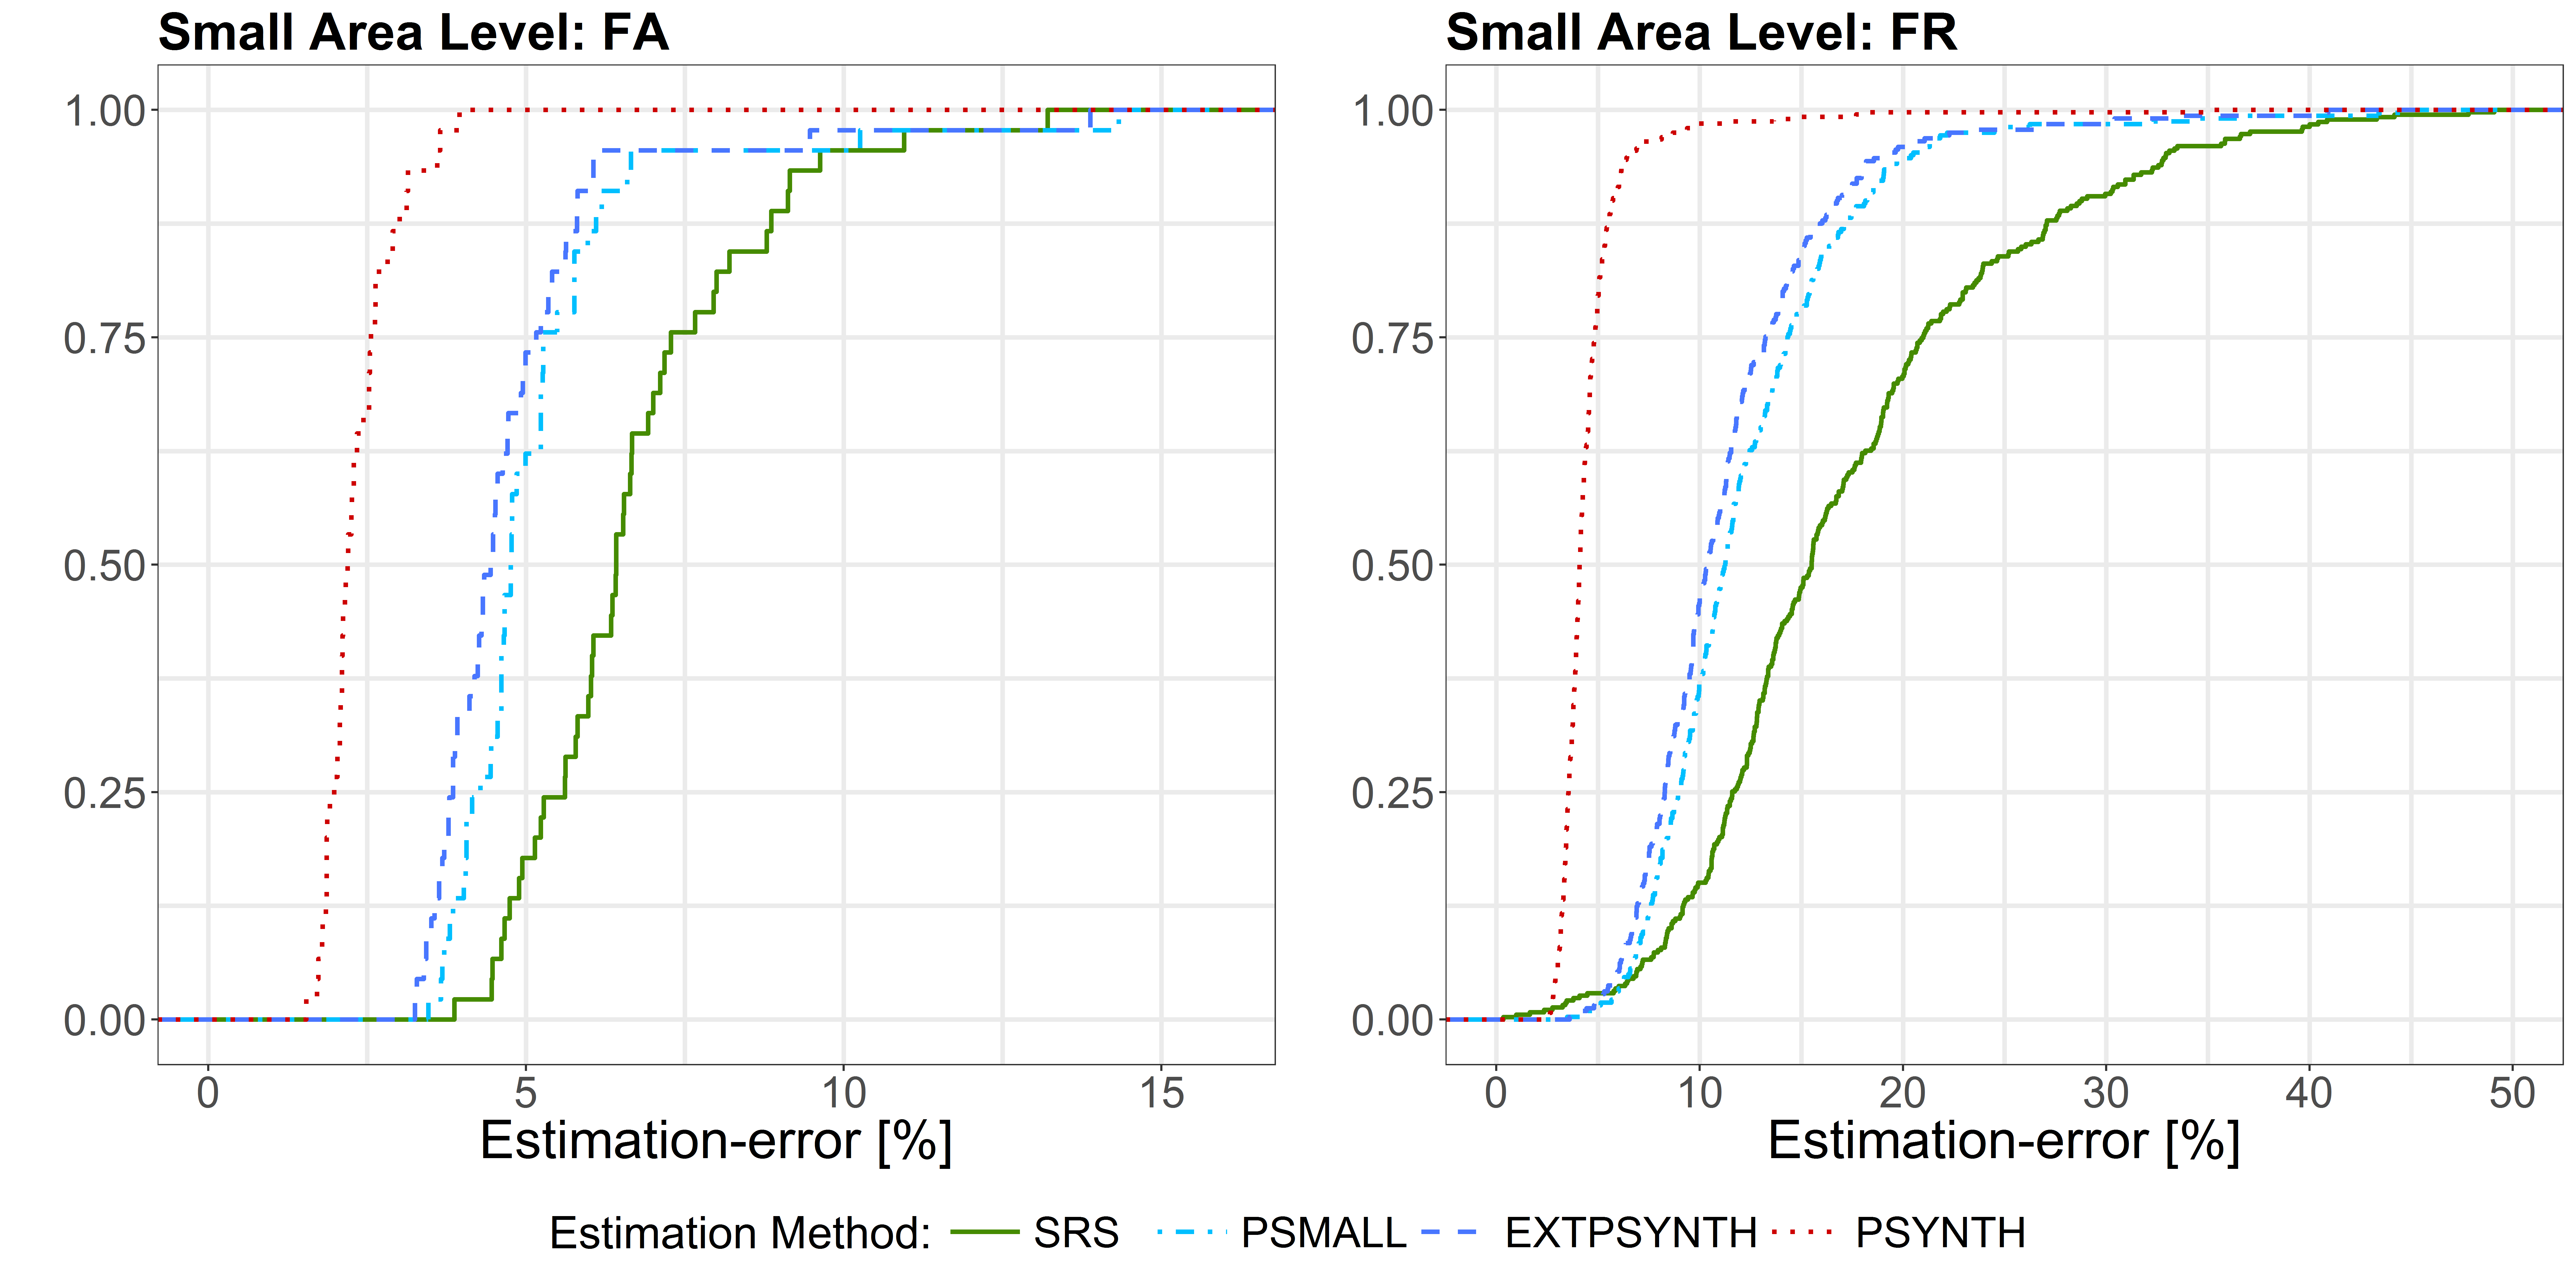
\includegraphics{fig/error_distr_foa_fu.png}}
	\caption{Cumulative distribution of estimation errors under SRS, \psmall{}, \extpsynth{} and the \psynth{} estimator. \textit{Left}: Results for the 45 FA units. \textit{Right}: Results for the 388 (SRS), 321 (\psmall{}, \extpsynth{}) and 403 (\psynth{}) FR units.}
	\label{fig:disterrors}
\end{figure}

On both small area levels, the \psynth{} estimator resulted in much smaller estimation errors compared to \psmall{} and \extpsynth{}. This was as expected, since the \psynth{} variance estimate does not take the residual variation in each small area unit into account (Section \ref{sec:psynth}). Compared to the asymptotically design-unbiased estimators \psmall{} and \extpsynth{}, the estimation errors produced by \psynth{} thus seem to be too optimistic. One should also recall that the estimates of the \psynth{} estimator are potentially design-biased.


% ----------------------------------------------------------------------- %
% ----------------------------------------------------------------------- %
\subsection{Comparison of \psmall{} and \extpsynth{}}
\label{sec:comp}

Figure \ref{fig:disterrors} reveals that the error distribution of \psmall{} and \extpsynth{} are very similar, with \psmall{} showing marginally higher estimation errors. In order to investigate the differences between \psmall{} and \extpsynth{}, we compared the g-weight variances of both estimators for all 321 FR units (Fig. \ref{fig:compvar}, left). As obvious, \psmall{} yielded slightly larger variances for the vast majority of the estimates. As addressed in Section \ref{sec:extpsynth}, one possible explanation for differences was the effect of one or more clusters not entirely being included in a small area unit, as this would constitute an assumption violation of the \extpsynth{} estimator. This violation was actually observed in 155 of the 321 FR units (48\%). We compared the variances of \psmall{} and \extpsynth{} for all small areas that did not have the violations using a Wilcoxon Signed-Rank Test \citep{wilcoxon1970} on a 5\% significance level. This test was also performed pairwise for groups $n_{2,G} \leq 6$, $n_{2,G} > 6$ and $n_{2,G} > 10$. The distribution of variances from \extpsynth{} was found to be highly significantly lower than that of \psmall{} except for the group of $n_{2,G} > 10$. The latter was expected since the variances of both estimators are asymptotically equivalent under large terrestrial sample sizes $n_{2,G}$ within the small area \citep[pp.17--18]{mandallaz2016}. This was also confirmed by a visual comparison of the absolute differences in the variances (Fig. \ref{fig:compvar}, right) which decreased with increasing terrestrial sample size. Performing the same comparison for small areas with violations also revealed the \extpsynth{} variances to be significantly smaller than the respective \psmall{} variances until sample sizes $n_{2,G} > 10$. Based on these investigations, it was not possible to determine whether the differences for sample sizes smaller than 10 were caused by the violations or just reflect the general tendency of \extpsynth{} to produce smaller variances than \psmall{} under small sample sizes. However, a visual inspection provided some evidence that the violations created a statistically significant influence on the \extpsynth{} variance (Fig. \ref{fig:compvar}, left, red diamonds) that makes it appear to be slightly over-optimistic. For sample sizes of $n_{2,G} < 6$, a weakly significant difference between the \extpsynth{} variances of those small areas with violations and the \extpsynth{} variances without violation was also indicated by an unpaired Wilcoxon Rank-Sum Test. However, the differences were still marginal and a comparison of the confidence intervals of \psmall{} and \extpsynth{} revealed that the variance differences did not lead to statistically significant point estimates.

\begin{figure}[H]
	\centering
	\resizebox{1\hsize}{!}{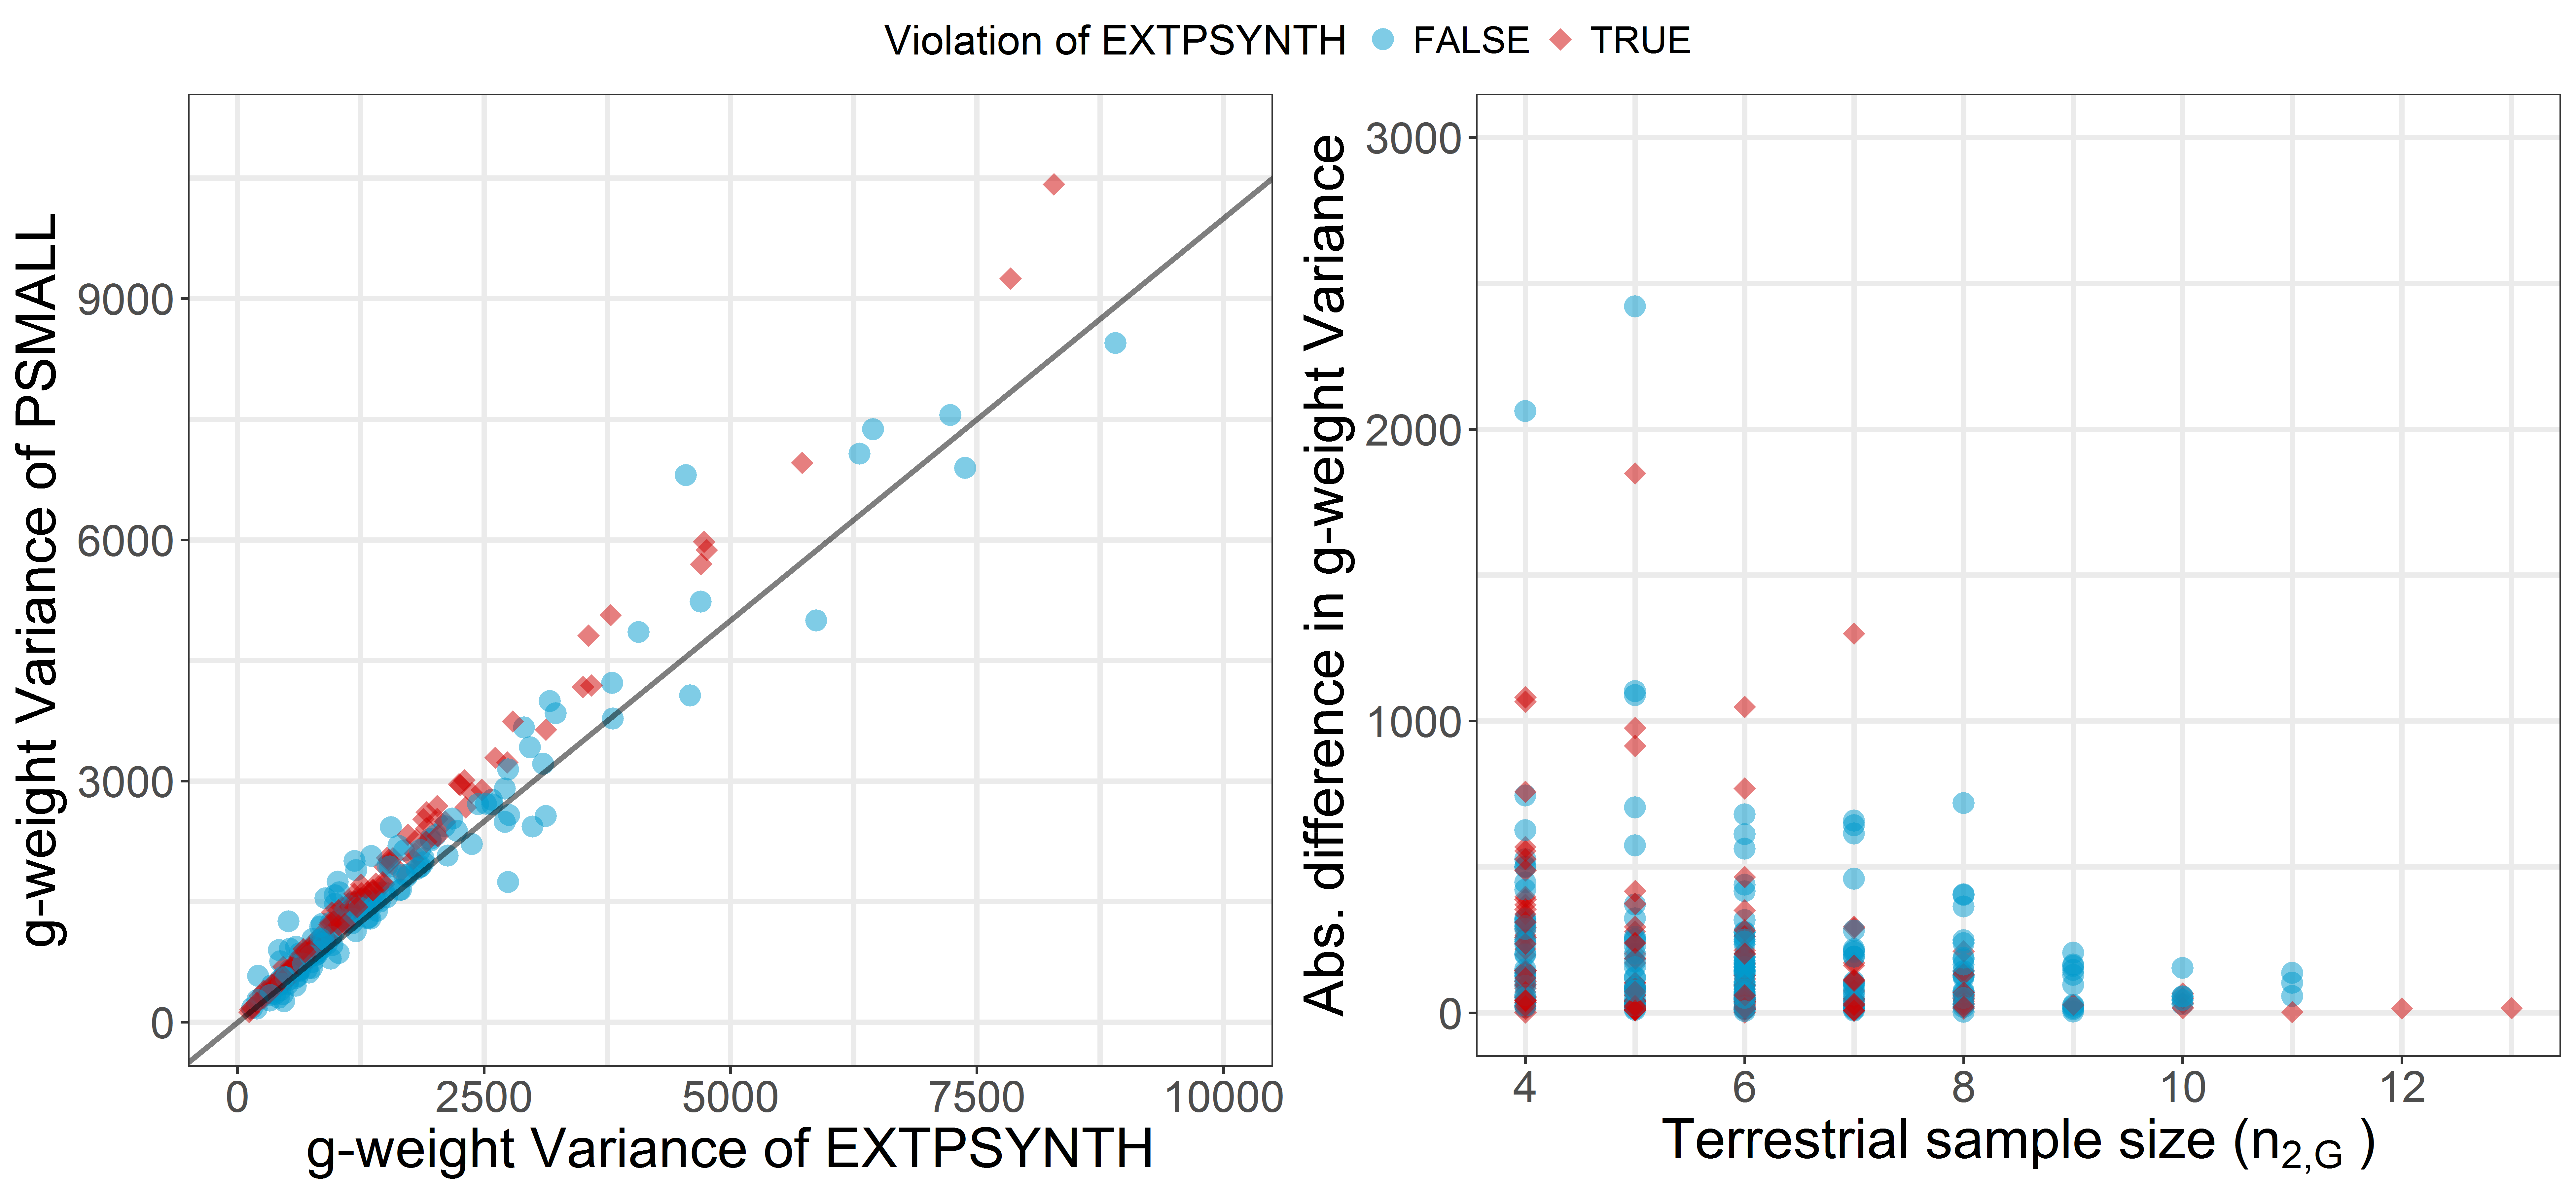
\includegraphics{fig/psmall_vs_extpsynth_fu.png}}
	\caption{\textit{Left}: Comparison of the g-weight variance between the PSMALL and the EXTPSYNTH estimator for the 321 FR units.
		\textit{Right}: Difference in g-weight variance between the PSMALL and the EXTPSYNTH estimator in dependence of the terrestrial data ($n_{2,G}$) in the FR unit.}
	\label{fig:compvar}
\end{figure}




% ----------------------------------------------------------------------- %
% ----------------------------------------------------------------------- %
\subsection{Variance reduction compared to SRS}
\label{sec:gain_eval}

The variance reduction relative to SRS for \psmall{} and \extpsynth{} are described in Figure \ref{fig:gain} and Table \ref{tab:gain}. A direct comparison of the variances within the small area units revealed that the application of the design-unbiased estimators (\psmall{}, \extpsynth{}) led to a variance reduction compared to SRS in all FA units. In 75\% of the FA units, the \extpsynth{} estimator was able to reduce the variance by up to 54.1\%. The reduction in variance can also be expressed in the relative efficiency values, which were 2.02 on average and ranged between 1.18 and 4.13 on the FA level. On FR level, the reduction in variance even reached values of 90\% and relative efficiencies of 30 (Table \ref{tab:gain} and Fig. \ref{fig:gain}). The \psmall{} estimator again yielded slightly lower variance reductions and relative efficiencies due to the generally smaller variances of the \extpsynth{} estimator (Section \ref{sec:comp}).

\begin{figure}[H]
	\centering
	\resizebox{0.73\hsize}{!}{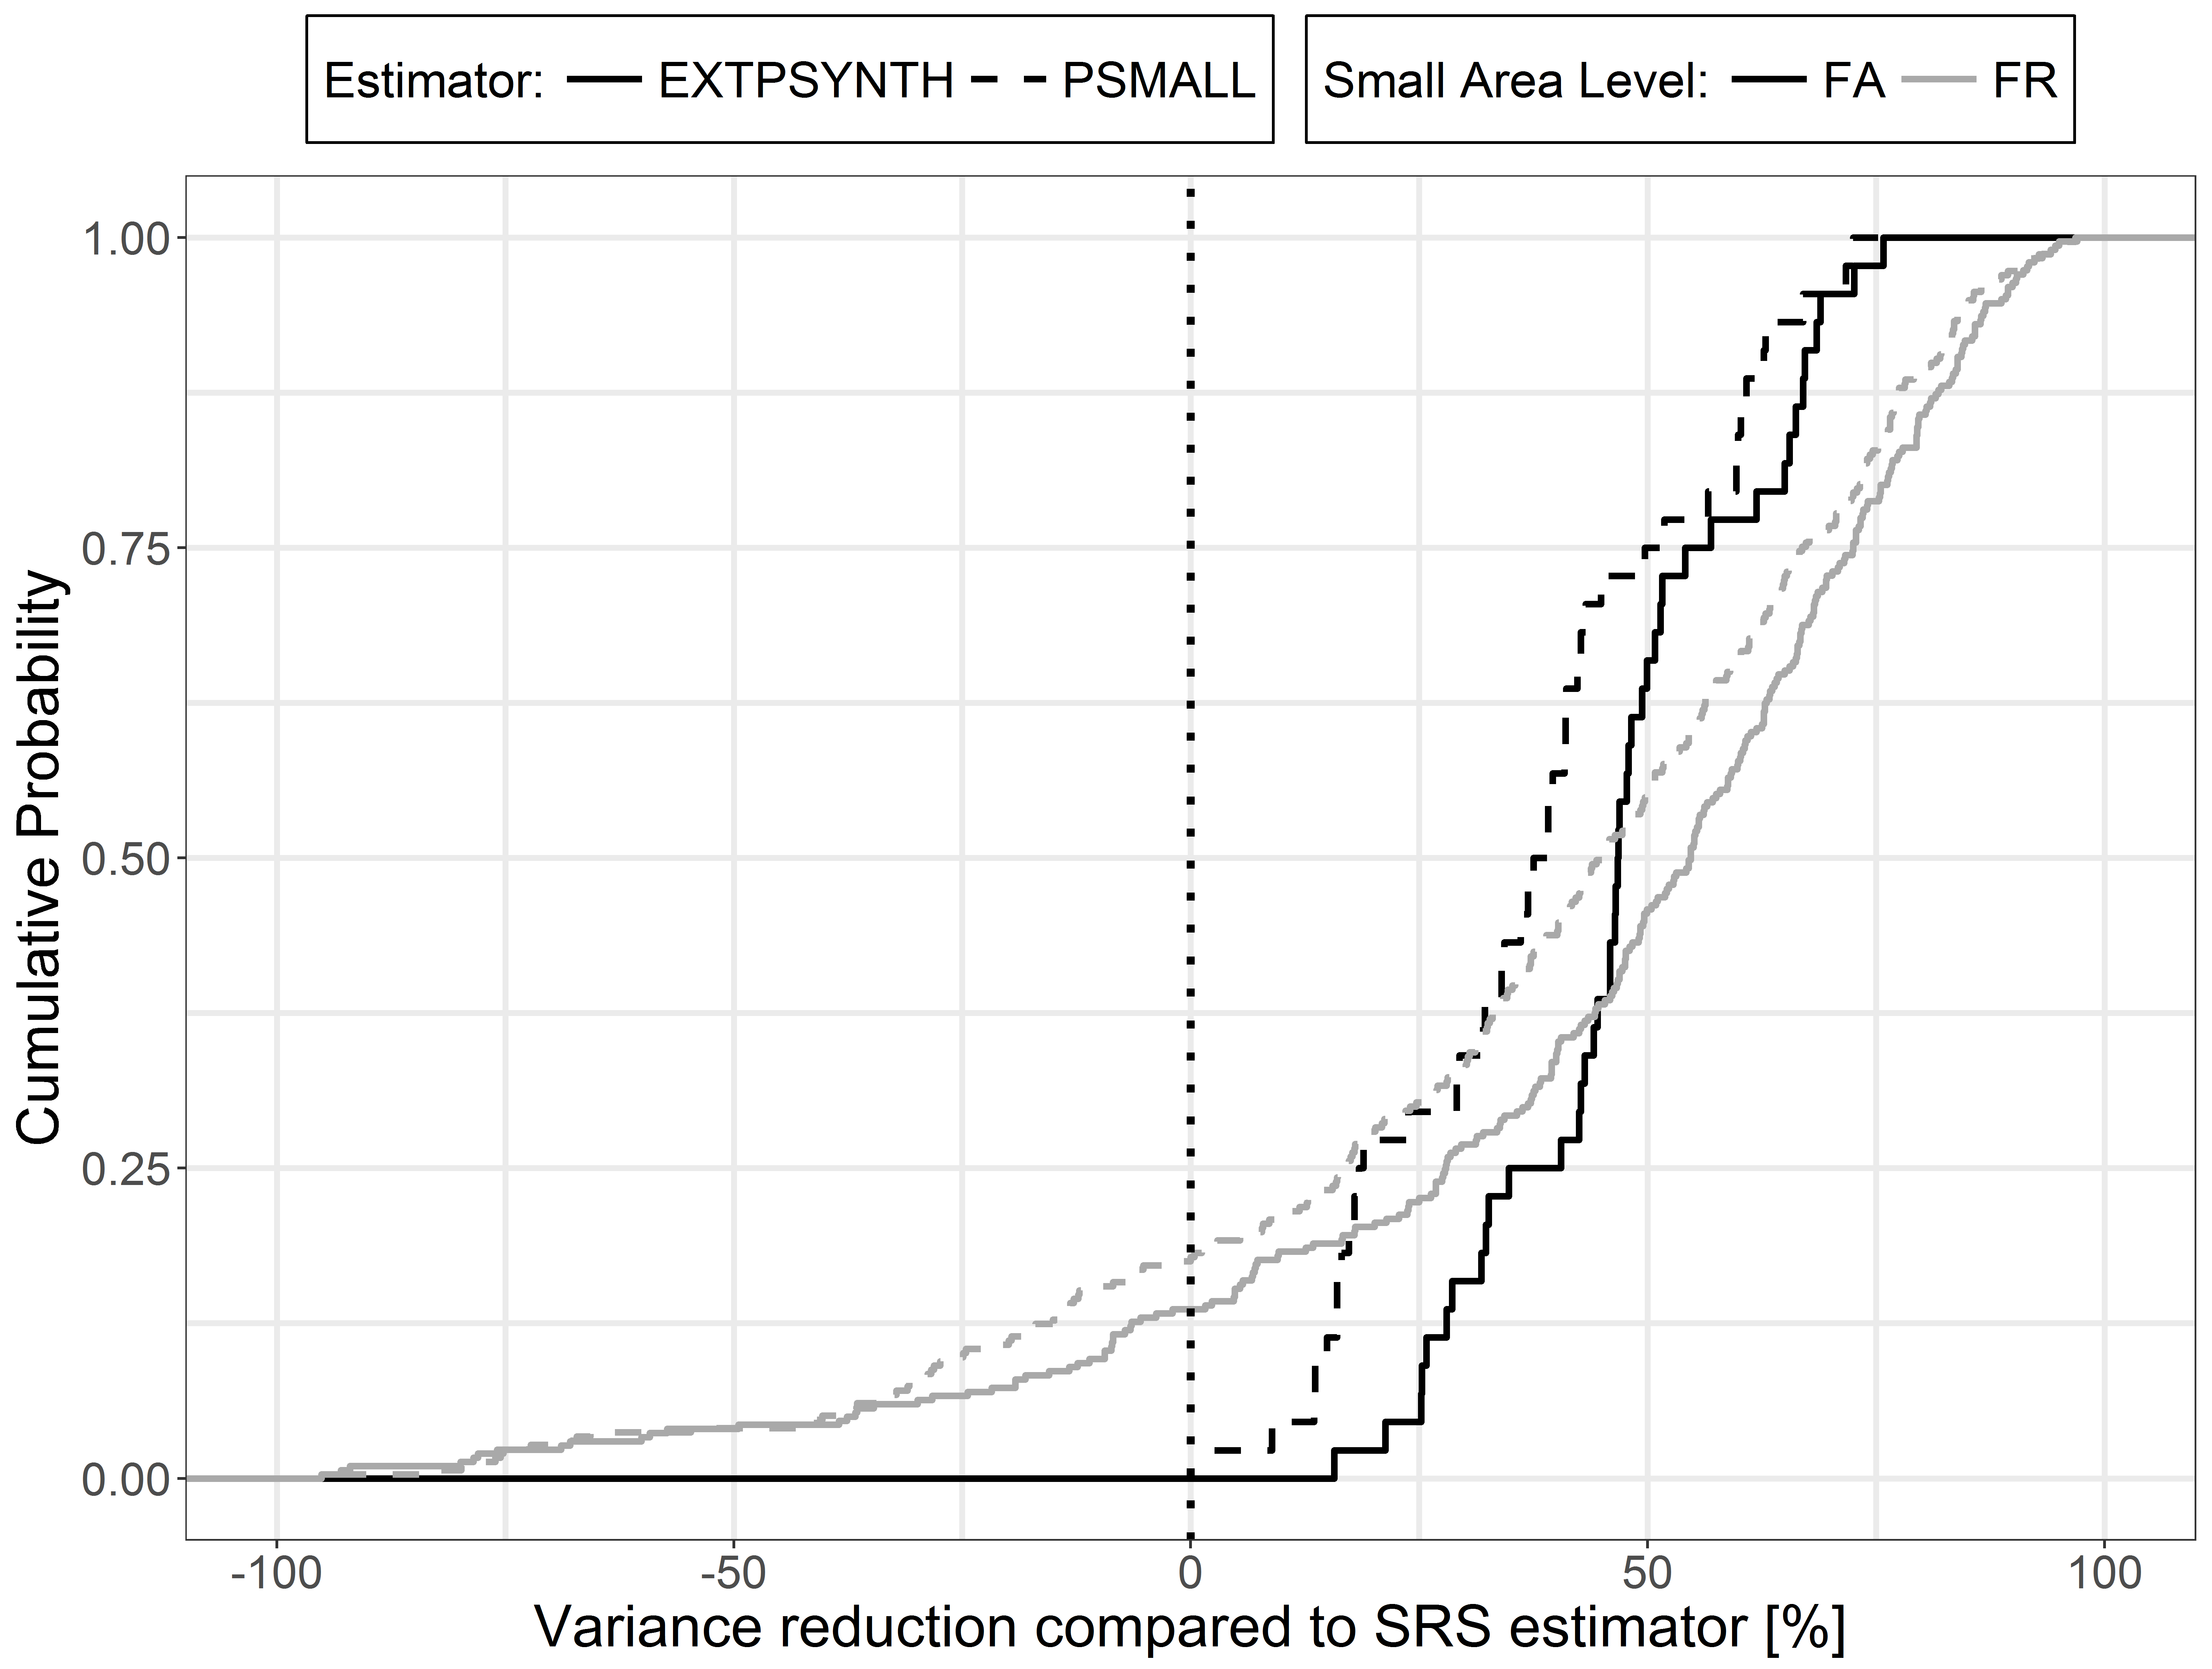
\includegraphics{fig/compare_onephase_extpsynth_psmall.png}}
	\caption{Cumulative distribution of variance reduction by the PSMALL and EXTPSYNTH compared to the SRS estimator for the  45 FA and 321 FR units.}
	\label{fig:gain}
\end{figure}

\begin{table}[H]
	\begin{center}
		\caption{Descriptive summary of variance reduction compared to SRS and relative efficiencies on the two forest district levels. $N_u$: number of evaluated small area units.}
		\vspace{0.2cm}
		\label{tab:gain}
		{\small %
			\begin{tabular}{c|l c|c c c|c c c} %8cols
				\hlineB{1}
				\multirow{2}{*}{District level} & \multicolumn{2}{c|}{\multirow{2}{*}{Estimator}} & \multicolumn{3}{c|}{Variance reduction [\%]} & \multicolumn{3}{c}{relative efficiency} \\
				\cline{4-9} & & & mean & min & max & mean & min & max \\
				\hline \hline
				\multirow{2}{*}{FA} & PSMALL    & ($N_u$=45)  & 33.51 &  2.6 & 72.5 & 1.74 & 1.03 & 3.64 \\
				& EXTPSYNTH & ($N_u$=45)  & 43.30 & 15.7 & 75.8 & 2.03  & 1.18 & 4.13 \\
				\hlineB{2}          
				\multirow{2}{*}{FR} & PSMALL    & ($N_u$=321) & 12.48 & -1203.9 & 96.8 & 2.54 & 0.08 & 31.61  \\
				& EXTPSYNTH & ($N_u$=321) & 24.75 & -892.7  & 97.0 & 2.95 & 0.10 & 33.70 \\
				\hline \hline
			\end{tabular}
		}%
	\end{center}
\end{table}

Cases also occurred on the FR level where one or both two-phase estimators produced larger variance values than under the SRS estimator. This happened in 19\% of the FR units under the \extpsynth{}, and in 24\% of the FR units under the \psmall{} estimator. One possible reason for this was supposed to be a large residual variance due to a poor performance of the regression model within the small area unit. In order to investigate this hypothesis, we analyzed the three variance terms of the \psmall{} estimator (Eq. \ref{eq:psmallvar}), i.e. the variance introduced by the uncertainty of the regression coefficients (term 1), the variance caused by estimating the auxiliary means (term 2), and the variance of the model residuals (term 3). In general, the residual term is expected to make the largest contribution to the overall variance since it's sample size is based on $n_{2,G}$ whereas the auxiliary term and the coefficient term are based on larger sample sizes, i.e. $n_{1,G}$ and $n_2$ respectively. Figure \ref{fig:fail} illustrates the share of the overall variance by the residual term of the \psmall{} estimator scaled by the overall percentage reduction or increase of the variance compared to SRS for various small area sample sizes $n_{2,G}$. Not surprisingly, the residual term generally constitutes the dominating part of the \psmall{} variance (around 84\% on average). It has to be noted that such high residual term dominance does not necessary indicate that the \psmall{} variance will be disproportionately large (Figure \ref{fig:fail}, \textit{right}). However, the vast majority of cases where the \psmall{} variance was considerably larger than the SRS variance occurred where the residual term contributed over 75\% to the overall \psmall{} variance (Figure \ref{fig:fail}, \textit{left}). Among those cases, the most pronounced were observed under small sample sizes $n_{2,G} < 5$. Here, the average increase in variance compared to SRS of those FR units with $n_{2,G}=4$ was 272\%, compared to 62\% for FR units with $n_{2,G} > 4$. In contrast, the decreases in variance compared to SRS (Figure \ref{fig:fail}, \textit{right}) were much more homogeneous in magnitude and also independent of the terrestrial sample size. Since $n_{2,G}$ is the same for \psmall{} and SRS, these observations imply that in the problematic small areas, the sum of square residuals for the regression model are likely larger than the sum of square local densities for the clusters in $s_{2,G}$. This indicates the presence of outliers with large residuals, which likely arise when there was forest loss after the ALS scanning but before the terrestrial survey year. % [check that]

\begin{figure}[H]
	\centering
	\resizebox{1\hsize}{!}{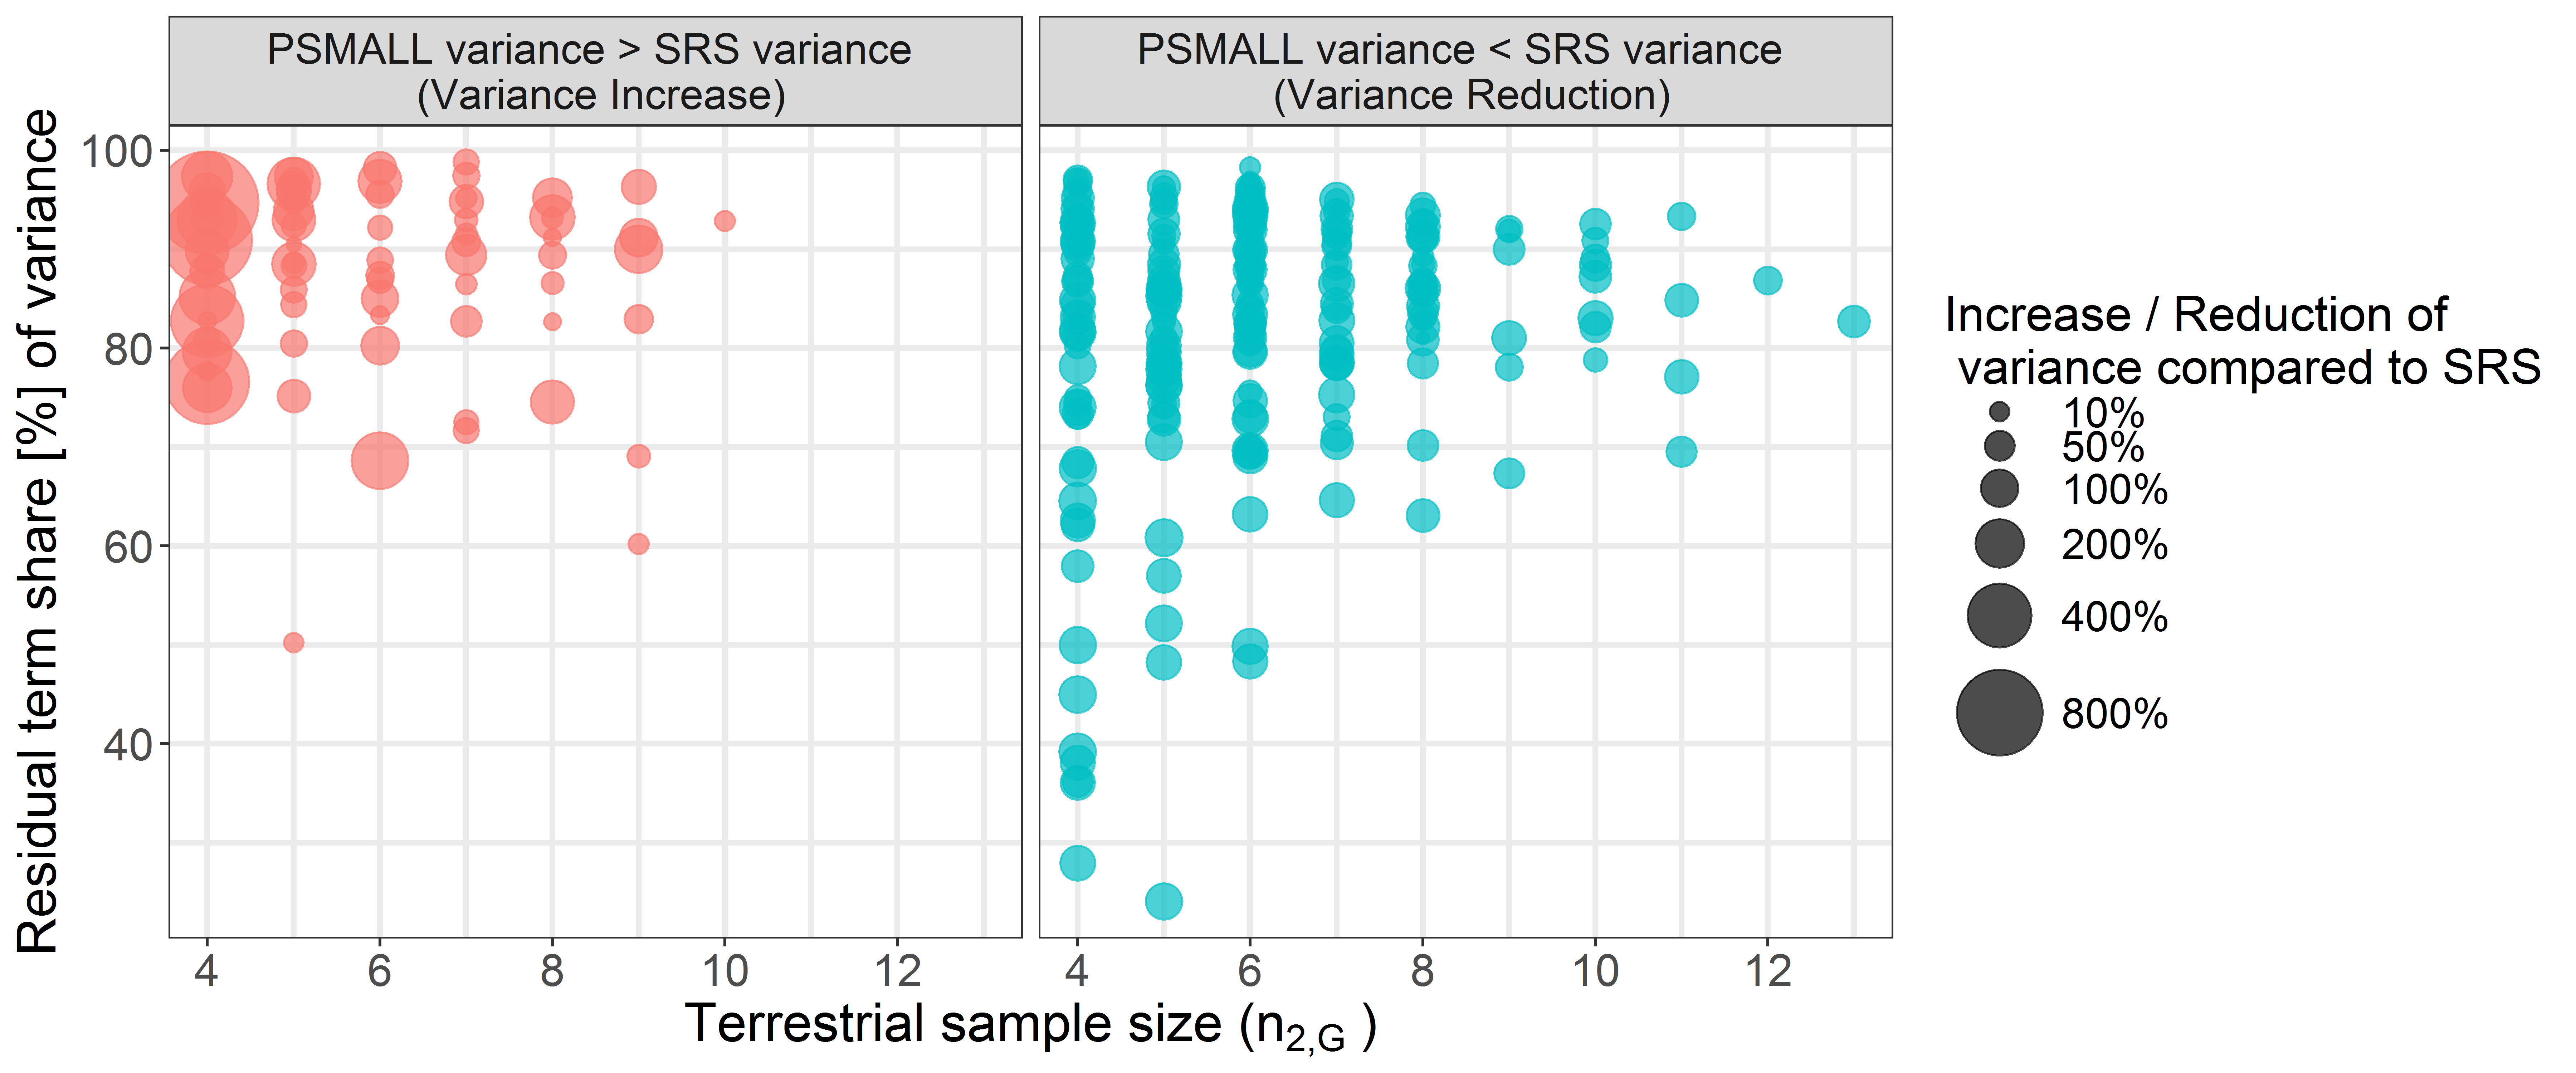
\includegraphics{fig/eval_2phase_fail_11.png}}
	\caption{Share of the overall variance by the residual term of the \psmall{} estimator for various small area sample sizes. Points are scaled by the overall percentage reduction/increase of the variance compared to SRS.}
	\label{fig:fail}
\end{figure}


%----------------------------------------------------------------------------------------------%
% ---------------------------------- Discussion ---------------------------------------------- %

\section{Discussion}
\label{sec:Dis}

% ------------------------ %
\subsection{Performance of estimators}

With the objective of extending the use of the German NFI data to additional estimation on small-scale management levels, we evaluated the performance of design-based small area regression estimators with respect to their suitability for future operational large scale application. For this reason, we conducted a case study in the German federal state of Rhineland-Palatinate where we applied the SRS, the \psmall{} and the \extpsynth{} estimators to produce estimates of the mean timber volume on two forest management levels over the entire federal state area, comprising 45 and 405 small area units respectively. In order to assess and compare the performance of the estimators, it was of particular interest to gather information about the magnitudes of estimation precision they can provide.\par

%Important criteria were considered to be:
%
%- the magnitude of estimation precision on the respective management level
%- the ability of the small area estimators to
%   a) be applied for large scale application, and 
%   b) be frequently repeated
%   c) be transferred / applicable to numerous forest attributes under comparable low effort
%   d) provide reliable specification of their estimation errors (uncertainties / precisions)
%- the identification of suitable auxiliary information, especially remote sensing data, with respect to their predictive power and their future availability

Our study showed that on both small area levels, the \psmall{} and the \extpsynth{} estimators generally led to a substantial reduction in estimation error compared to the standard one-phase SRS estimator. On the upper management level (FA districts), \psmall{} and \extpsynth{} produced estimation errors smaller than 5\% for 73\% of the small areas compared to only 17\% under the one-phase SRS estimator. The same level of precision could not be achieved on the lower management level (FR districts) primarily due to substantially smaller terrestrial sample sizes. However, in 95\% of the FR units, the estimation errors could be limited to 20\% compared to 40\% under SRS. A pairwise comparison of the confidence intervals revealed that the estimators did not produce significantly different point estimates. The much smaller estimation errors of the \psynth{} estimator reflected the fact that it does not try to correct for potential bias in the point estimate which can lead to overly optimistic estimation errors and confidence intervals. One should thus prefer the unbiased estimates of \psmall{} or \extpsynth{} whenever their calculation is possible.\par

For several FR units, it was observed that the \psmall{} and the \extpsynth{} estimator can occasionally produce larger variances than the SRS estimator. It is important to note that this is in perfect agreement with the theory of both two-phase estimators and can theoretically appear if the residual variance in the small area, which generally constitutes the dominating part of the two-phase variance, turns out to be much higher than the variance of the terrestrial data in the small area. The empirical findings of our study suggest that such cases can particularly occur if moderate or poor model fits within a small area are combined with small terrestrial sample sizes ($\leq 5$) in the small area. A closer look on these small areas thus might reveal the reason for the poor prediction performance and help to improve the model fit. Nonetheless, it should be kept in mind that small terrestrial sample sizes can also cause the SRS estimator to not reflect the actual variation of the local density within a small area. In this case, the two-phase variance estimate might be larger but more realistic. Whereas a visual analysis of aerial images, remote sensing data or stand maps might give some further evidence for or against this hypothesis, a definite proof is practically infeasible.\par

We were also able to empirically confirm that the \extpsynth{} estimator generally produces slightly smaller variances and estimation errors than the \psmall{} estimator. This is most probably caused by marginally smaller model residuals due to the intercept adjustment to the terrestrial data in the small area unit, which is primarily a means to ensure the zero mean residual property of the \extpsynth{} estimator. However, our analysis indicated that the difference between the two estimators is negligible for sample sizes $\geq$ 10 due to their asymptotic equivalency. We further investigated a potential impact on the \extpsynth{} variance caused by the assumption violation that one or more clusters are not entirely included in the small area unit and found a slight but statistically significant tendency to be over-optimistic for sample sizes smaller than 6. More empirical evidence must be gathered before generalizing this as a rule of thumb for the application of the \extpsynth{} under cluster sampling. It thus seems recommendable to prefer the \extpsynth{} to the \psmall{} estimator if its assumptions are not violated since it yields slightly smaller variances under mathematically soundness. Even if the differences between both estimators were marginal and did not lead to significantly different point estimates, \psmall{} can serve as a safe alternative if the \extpsynth{} assumption is violated. Aside from this, calculating both \psmall{} and \extpsynth{} and subsequently compare their results is always recommended to reveal suspicious deviations.\par


% ------------------------ %
\subsection{Auxiliary data}

The auxiliary data used in our study were derived from two remote sensing sources, i.e. an ALS canopy height model and a tree species classification map. Likewise in many similar studies, the ALS mean canopy height proved to be the explanatory variable with highest predictive power. However, the large time-gaps of up to 10 years between the ALS acquisition and the terrestrial survey date caused the substantial introduction of artificial noise in the data. Whereas a post-stratification to the ALS acquisition years was an effective means to counteract the implied residual inflation, several leverage points were unambiguously caused by the temporal asynchronicity. Undetectable forest loss during the gap between the ALS acquisition and the NFI was also likely a cause for high residual variance in some small area units compared to the terrestrial data variance, which subsequently led to higher variances than the SRS estimator. As opposed to the ALS data, the availability of a country-wide tree species classification map has yet been unique among all German federal states. Whereas the study of \citet{hill2017a} already showed that the tree species information was able to improve the model fit, it has yet not been used to its full potential. One reason for this was the impossibility of modeling individual tree species within each ALS acquisition year, which would add further explanatory power. Another reason was the lack of available satellite data for classification in some parts of the country, which led to missing values in the inventory data and restricted 19 FR units to a simpler regression model. Promising steps with respect to more up-to-date canopy height information have already been made, as the topographic survey institution of RLP will from this year on provide a country-wide canopy height model derived from aerial imagery acquisitions. These campaigns will in the future be conducted in a two-year period and allow to derive canopy height information matching the dates of terrestrial forest inventories. A study of \citet{kirchhoefer2017} recently indicated that similar model performance for German NFI data can be achieved using such imagery-based canopy height models. Additionally, the improved coverage and repetition rate of the Sentinel-2 satellite \citep{sentinel2} will allow to produce annually updated tree species classification maps. We consider these alternative auxiliary data sources to also solve the problem of missing explanatory variables at inventory plots. One could also make use of the exhaustive information within the two-phase estimators by using the true auxiliary means \citep{mandallaz2013a, mandallaz2013b}, which could further decrease estimation errors. Previous studies of \citet{mandallaz2013b} however showed that given a reasonable large sample size of the first phase, the differences in the estimation error are usually small. With respect to the substantial improvements in the temporal synchronicity between auxiliary and terrestrial inventory data, we consider the demonstrated double-sampling approach also to be very efficient for the estimation of change \citep{massey2015b}.\par


%----------------------------------------------------------------------------------------------%
% ---------------------------------- Conclusion ---------------------------------------------- %

\section{Conclusion}
\label{sec:concl}

The study led to two major conclusions: (1) the \extpsynth{} and \psmall{} estimator generally achieved substantially smaller estimation errors on the two investigated forest district levels compared to the SRS estimator. Thus, the demonstrated small area estimation procedure constitutes a major contribution to an additional use of the German NFI data for estimation below the federal state level. Further close cooperation with the forest authorities is crucial to evaluate whether the achieved error levels are already sufficient enough in order to support forest planning decisions. A first study will concentrate on testing the \extpsynth{} and \psmall{} confidence intervals as a validation source for the stand-wise inventories. (2) Despite the quality restrictions, the ALS data and the tree species map were found to be well suited to model the mean timber volume on the plot and cluster level. With the prospect of more frequently updated aerial canopy height models and tree species maps, the two data sources will become even more attractive to be used as an integral part of future operational applications. The improving availability of remote sensing data will also allow to extent the demonstrated estimation procedure to the estimation of change. We consider this to be one of the next milestones towards a future operational use of the demonstrated small area estimation procedure.




%%%%%%%%%%%%%%%%%%%%%%%%%%%%%%%%%%%%%%%%%%%
\vspace{6pt} 
%
%
%%%%%%%%%%%%%%%%%%%%%%%%%%%%%%%%%%%%%%%%%%%
\acknowledgments{We want to express our gratitude to Prof. H. Heinimann (Chair of Land Use Engineering, ETH Zurich) for supporting this study. We also want to explicitly thank Dr. Johannes Stoffels and Dr. Henning Buddenbaum from the Environmental Sensing and Geoinformatic Group of University of Trier for providing the ALS data and tree species classification map, and Dr. Kai Husmann and Dr. Christoph Fischer from the Northwest German Forest Research Institution G{\"o}ttingen for their advice in processing the terrestrial inventory data. Special gratitude is also owed to Dr. Thomas Riedel from the Th{\"u}nen Institute for providing the densified NFI sample grid, and Dr. Alexander Massey for proofreading.}
%
%%%%%%%%%%%%%%%%%%%%%%%%%%%%%%%%%%%%%%%%%%%
\authorcontributions{Andreas Hill conducted the study and wrote the manuscript. Daniel Mandallaz developed the design-based estimators and supported the statistical analysis. Joachim Langshausen supported the study on the part of the State Forest Service Rhineland-Palatinate and cross-checked the analysis and the manuscript.}
%
%%%%%%%%%%%%%%%%%%%%%%%%%%%%%%%%%%%%%%%%%%%
\conflictsofinterest{The authors declare no conflict of interest.} 


%%%%%%%%%%%%%%%%%%%%%%%%%%%%%%%%%%%%%%%%%%
%% optional
\appendixtitles{no} %Leave argument "no" if all appendix headings stay EMPTY (then no dot is printed after "Appendix A"). If the appendix sections contain a heading then change the argument to "yes".
\appendixsections{one} %Leave argument "multiple" if there are multiple sections. Then a counter is printed ("Appendix A"). If there is only one appendix section then change the argument to "one" and no counter is printed ("Appendix").
\appendix

\section{}
% -------------------------------------- %
\subsection*{R-squared on cluster level}

The R$^2$ on the cluster level is calculated using the number of plots $M(x)$ of each cluster in order to weight for the varying number of plots on which $Y_c(x)$ and $\hat{Y}_{c}(x)$ are based on. 

\begin{equation*}\label{eq:R_squared_clust}
R^2 =  \frac{\sum_{x \in s_2} \Big(\frac{M(x)}{\bar{M_2}}\Big)^2 \Big(\hat{Y}_{c}(x)-\hat{\bar{Y}}_c\Big)^2}{\sum_{x \in s_2} \Big(\frac{M(x)}{\bar{M_2}}\Big)^2 \Big(Y_{c}(x)-\hat{\bar{Y}}_c\Big)^2}
\end{equation*}

\noindent $Y_c(x)$ and $\hat{Y}_{c}(x)$ are the predicted and observed local densities on the cluster level calculated according to Equations \ref{eq:locdens_clust} and \ref{eq:globresids}. $\hat{\bar{Y}}_c$ is the estimated sample mean corresponding to the weighted mean over all observed local densities on the cluster level (Eq. \ref{eq:srs_est_clusters}).\par

% -------------------------------------- %
\subsection*{RMSE on cluster level}

The same weights $M(x)$ are also applied to calculate the RMSE on the cluster level. $n_2$ is the number of clusters used in the modeling frame.

\begin{equation*}\label{eq:RMSE_clust}
RMSE= \sqrt{\frac{1}{n_{2}}  \sum_{x \in s_2} \Big(\frac{M(x)}{\bar{M}_2}\Big)^2 \Big(\hat{Y}_{c}(x)-Y_c(x)\Big)^2}
\end{equation*}

\noindent The \textit{relative} or \textit{normalized} RMSE is calculated by dividing the RMSE by the estimated sample mean $\hat{\bar{Y}}_c$:

\begin{equation*}\label{eq:NRMSE_clust}
RMSE[\%] = \frac{RMSE}{\hat{\bar{Y}}_c}
\end{equation*}

\noindent Note that the weights $\frac{M(x)}{\bar{M_2}} \equiv 1$ if the number of plots per cluster is constant.


%%%%%%%%%%%%%%%%%%%%%%%%%%%%%%%%%%%%%%%%%%
% Citations and References in Supplementary files are permitted provided that they also appear in the reference list here. 

%=====================================
% References, variant A: internal bibliography
%=====================================
\reftitle{References}
\externalbibliography{yes}
\bibliography{bib/literaturerRLPsae}

\end{document}

